\documentclass[11pt]{article}
\usepackage[a4paper,margin=2cm]{geometry}
\usepackage[utf8]{inputenc}
\usepackage[T1]{fontenc}
\usepackage{lmodern,amsmath,amssymb,booktabs,longtable,graphicx,array,url,makecell}
\renewcommand{\cellalign}{bl}\renewcommand{\theadalign}{bl}
\usepackage[hidelinks]{hyperref}
\renewcommand{\thetable}{S\arabic{table}}
\renewcommand{\thefigure}{S\arabic{figure}}
\setlength{\LTcapwidth}{\textwidth}
\title{Supplementary material for\\``Phase-Dependent False-Alarm Calibration and Its Transport Across Engines in Full-Flight Aero-Engine Anomaly Detection''}
\author{Jinghang Mei}
\date{}
\begin{document}
\maketitle

\noindent This supplement accompanies the article. Every table is a formatted view of committed outputs of the frozen
and post-confirmation analyses; values are rounded for display and nothing is recomputed. Healthy false-positive rates
(FPR) are percentages of healthy rows; differences are in percentage points (pp). Runs are one PCA run (PCA) and three
seeds each of Isolation Forest (IF s0--s2) and the past-only LSTM (LSTM s0--s2). Arms: P, pooled; C, retrospective
phase-conditioned; C$'$, past-only regime-conditioned; Q, continuous contextual baseline (healthy side only). The primary
nominal target is 1\%. Machine-readable versions of all tables are in the public repository
(\url{https://github.com/surnamemei/ncmapss-phase-entanglement}; \texttt{results/} and \texttt{paper/mssp/evidence/}).

\tableofcontents
\bigskip

\section{Provenance, reproduction and deviations}
The study was staged: DS02 exploratory discovery, a protocol freeze, a one-shot frozen DS03 confirmation, and two
post-confirmation stages (protocol v1.0 and the adversarial-validation plan), each committed before execution.
Before every post-confirmation run, reproduction gates required exact agreement with the frozen evidence:
rescored healthy score vectors equalled the frozen fingerprints bit for bit; recomputed healthy count tables,
calibration-only $\kappa$ locks and bootstrap summaries equalled the committed outputs; and the committed per-flight
alarm fractions reproduced every committed detection delay. A hash manifest of 186 frozen files was verified before
and after every run. Abnormal-state ($hs = 0$) rows were read once per dataset, after the calibration-only lock, and
never again. Table~\ref{tab:s1_provenance} lists the governing documents and records.

\paragraph{Deviations and amendments.}
(i) Amendment A-1 corrected a repository-metadata statement about the published v1.0.0 release tag; it was recorded
before any abnormal-state row was opened and changed no analysis. (ii) Dev-1: the error decomposition (Section~\ref{sec:adversarial}) was added after the plan and is
descriptive. (iii) Dev-2: operational definitions of the target-robustness claims were fixed in code before execution.
(iv) Dev-3: after all runs, an output guard and a robustness fix for phases without rows were added to the analysis
module; no output was regenerated, and every output names the module version that produced it. (v) Story-lock
Amendment 1 corrected the count of audit engines from flight classes absent from calibration (four, three of them
class 1) without changing any analysis.

\paragraph{Verification.} The repository's test suite re-derives the post-confirmation metrics and operating points
from committed inputs, and a checker re-derives every number cited in the article and verifies that it appears
verbatim.

\begin{footnotesize}
\begin{longtable}{p{0.27\textwidth}p{0.44\textwidth}l}
\caption{Provenance of the analyses reported in the article. Each run record also names the analysis-module version that produced its outputs.}\label{tab:s1_provenance}\\
\toprule
Artefact & Path & SHA-256 (first 16 hex) \\
\midrule
\endfirsthead
\multicolumn{3}{l}{\emph{(continued)}}\\
\toprule
Artefact & Path & SHA-256 (first 16 hex) \\
\midrule
\endhead
\bottomrule
\endfoot
Frozen baseline manifest (186 files) & \path{docs/mssp/frozen_baseline.sha256} & \texttt{37c0cef26826bef2} \\
\midrule
Post-confirmation protocol v1.0 & \path{docs/mssp/post_confirmation_mitigation_protocol.md} & \texttt{b4a669cdd00d4075} \\
\midrule
Protocol amendments & \path{docs/mssp/AMENDMENTS.md} & \texttt{60522a5b4eb5be60} \\
\midrule
Adversarial validation plan & \path{docs/mssp/adversarial_validation_plan.md} & \texttt{d993dd3f9e5ab286} \\
\midrule
Final story lock & \path{docs/mssp/FINAL_STORY_LOCK.md} & \texttt{f6c5b2cf2d067ed0} \\
\midrule
Post-confirmation module & \path{src/mssp_mitigation.py} & \texttt{2764f27113a0c7af} \\
\midrule
Adversarial-validation module & \path{src/mssp_adversarial.py} & \texttt{0b2db2b4ad60e509} \\
\midrule
DS02 endpoint record (abnormal rows read once) & \path{results/mssp_mitigation/ds02/stage_e/stage_e_record.json} & \texttt{a2ecfaa0eea41074} \\
\midrule
DS03 endpoint record (abnormal rows read once) & \path{results/mssp_mitigation/ds03/stage_e/stage_e_record.json} & \texttt{e95e80c76d154ec7} \\
\midrule
DS02 adversarial run record (A--C) & \path{results/mssp_adversarial/ds02/run_record_ABC.json} & \texttt{f676c2189422e2b8} \\
\midrule
DS03 adversarial run record (A--C) & \path{results/mssp_adversarial/ds03/run_record_ABC.json} & \texttt{5fdd9e77f976964c} \\
\midrule
DS02 baseline run record (D) & \path{results/mssp_adversarial/ds02/run_record_D.json} & \texttt{df0d765dd5ed67dd} \\
\midrule
DS03 baseline run record (D) & \path{results/mssp_adversarial/ds03/run_record_D.json} & \texttt{1c48684e825e8c9c} \\
\midrule
Adversarial summary record & \path{results/mssp_adversarial/summary/summary_record.json} & \texttt{1a59f7170292eead} \\
\end{longtable}
\end{footnotesize}


\section{Frozen discovery and confirmation}
The values in this section are the frozen DS02 (exploratory) and DS03 (frozen confirmation) results, shown unchanged.

\begin{footnotesize}
\begin{longtable}{lrrrrr}
\caption{Frozen DS02 PCA correction sensitivity (exploratory): pooled healthy FPR (\%) by phase at the 1\% target, primary phase rule, and worst off-diagonal cross-phase transfer FPR (\%).}\label{tab:s2_correction}\\
\toprule
Correction & Overall & Climb & Cruise & Descent & Worst transfer \\
\midrule
\endfirsthead
\multicolumn{6}{l}{\emph{(continued)}}\\
\toprule
Correction & Overall & Climb & Cruise & Descent & Worst transfer \\
\midrule
\endhead
\bottomrule
\endfoot
static & 1.277 & 0.146 & 0.583 & 3.001 & 14.306 \\
\midrule
static-derivative & 1.239 & 0.061 & 0.457 & 3.106 & 15.865 \\
\midrule
history & 1.363 & 0.125 & 0.428 & 3.459 & 15.555 \\
\end{longtable}
\end{footnotesize}

\begin{footnotesize}
\begin{longtable}{lrrrrr}
\caption{Frozen DS02 alternative retrospective phase rule (exploratory; 85\% altitude range and centred 60-s altitude rate at most 2 ft/s): pooled healthy FPR (\%) at the 1\% target.}\label{tab:s3_alternative_rule}\\
\toprule
Run & Climb & Cruise & Descent & Descent $-$ climb (pp) & Descent $-$ cruise (pp) \\
\midrule
\endfirsthead
\multicolumn{6}{l}{\emph{(continued)}}\\
\toprule
Run & Climb & Cruise & Descent & Descent $-$ climb (pp) & Descent $-$ cruise (pp) \\
\midrule
\endhead
\bottomrule
\endfoot
PCA & 0.131 & 0.270 & 3.563 & +3.432 & +3.293 \\
\midrule
IF s0 & 0.276 & 0.379 & 2.515 & +2.238 & +2.135 \\
\midrule
IF s1 & 0.247 & 0.387 & 2.787 & +2.540 & +2.400 \\
\midrule
IF s2 & 0.259 & 0.396 & 2.629 & +2.370 & +2.233 \\
\midrule
LSTM s0 & 0.451 & 0.516 & 2.264 & +1.813 & +1.747 \\
\midrule
LSTM s1 & 0.459 & 0.524 & 2.316 & +1.857 & +1.792 \\
\midrule
LSTM s2 & 0.530 & 0.540 & 2.270 & +1.741 & +1.730 \\
\end{longtable}
\end{footnotesize}

\begin{footnotesize}
\begin{longtable}{llrrrll}
\caption{Frozen individual-run pooled healthy FPR (\%) at the 1\% target with hierarchical (engine, then flight) bootstrap 95\% intervals for the contrasts (2000 replicates, thresholds re-estimated). Intervals belong to individual runs; no seed-mean interval exists.}\label{tab:s4_runs_intervals}\\
\toprule
Dataset & Run & Climb & Cruise & Descent & Descent $-$ climb, 95\% CI (pp) & Descent $-$ cruise, 95\% CI (pp) \\
\midrule
\endfirsthead
\multicolumn{7}{l}{\emph{(continued)}}\\
\toprule
Dataset & Run & Climb & Cruise & Descent & Descent $-$ climb, 95\% CI (pp) & Descent $-$ cruise, 95\% CI (pp) \\
\midrule
\endhead
\bottomrule
\endfoot
DS02 & PCA & 0.125 & 0.428 & 3.459 & +3.335 [+2.070, +5.629] & +3.031 [+1.808, +5.261] \\
 & IF s0 & 0.285 & 0.566 & 2.335 & +2.050 [+0.850, +4.074] & +1.769 [+0.678, +3.749] \\
 & IF s1 & 0.253 & 0.528 & 2.669 & +2.416 [+1.313, +4.166] & +2.141 [+1.012, +3.943] \\
 & IF s2 & 0.266 & 0.580 & 2.455 & +2.190 [+1.063, +3.947] & +1.875 [+0.742, +3.709] \\
 & LSTM s0 & 0.452 & 0.707 & 2.078 & +1.626 [+0.317, +2.838] & +1.371 [+0.528, +2.490] \\
 & LSTM s1 & 0.474 & 0.731 & 2.102 & +1.628 [$-$0.022, +2.817] & +1.372 [+0.399, +2.454] \\
 & LSTM s2 & 0.539 & 0.750 & 2.060 & +1.521 [$-$0.347, +2.802] & +1.309 [+0.330, +2.511] \\
\midrule
DS03 & PCA & 0.877 & 0.912 & 1.977 & +1.100 [+0.434, +1.785] & +1.066 [+0.560, +1.573] \\
 & IF s0 & 0.417 & 1.095 & 2.166 & +1.749 [+0.901, +2.847] & +1.071 [+0.404, +1.994] \\
 & IF s1 & 0.399 & 1.060 & 2.127 & +1.728 [+0.891, +2.833] & +1.067 [+0.426, +1.976] \\
 & IF s2 & 0.412 & 1.157 & 2.134 & +1.722 [+0.871, +2.772] & +0.976 [+0.347, +1.862] \\
 & LSTM s0 & 0.759 & 1.795 & 2.231 & +1.472 [+0.536, +2.870] & +0.436 [$-$0.222, +1.201] \\
 & LSTM s1 & 0.719 & 1.890 & 2.220 & +1.501 [+0.512, +3.022] & +0.330 [$-$0.270, +1.158] \\
 & LSTM s2 & 0.774 & 1.982 & 2.193 & +1.419 [+0.379, +3.059] & +0.210 [$-$0.582, +1.025] \\
\end{longtable}
\end{footnotesize}

\begin{footnotesize}
\begin{longtable}{lllrrrrr}
\caption{Frozen per-engine pooled-threshold healthy FPR (\%) at the 1\% target (DS02 exploratory; DS03 frozen confirmation). Directional exceptions remain visible.}\label{tab:s5_per_engine}\\
\toprule
Dataset & Run & Engine & Climb & Cruise & Descent & Descent $-$ climb (pp) & Descent $-$ cruise (pp) \\
\midrule
\endfirsthead
\multicolumn{8}{l}{\emph{(continued)}}\\
\toprule
Dataset & Run & Engine & Climb & Cruise & Descent & Descent $-$ climb (pp) & Descent $-$ cruise (pp) \\
\midrule
\endhead
\bottomrule
\endfoot
DS02 & PCA & 11 & 0.097 & 0.406 & 2.780 & +2.683 & +2.374 \\
 &  & 14 & 0.294 & 0.491 & 4.972 & +4.678 & +4.481 \\
 &  & 15 & 0.113 & 0.425 & 3.666 & +3.553 & +3.241 \\
 & IF s0 & 11 & 0.091 & 0.371 & 2.234 & +2.143 & +1.863 \\
 &  & 14 & 1.487 & 1.351 & 2.510 & +1.024 & +1.159 \\
 &  & 15 & 0.197 & 0.393 & 2.396 & +2.199 & +2.003 \\
 & IF s1 & 11 & 0.082 & 0.304 & 2.348 & +2.266 & +2.044 \\
 &  & 14 & 1.291 & 1.393 & 3.287 & +1.996 & +1.894 \\
 &  & 15 & 0.180 & 0.352 & 2.824 & +2.644 & +2.473 \\
 & IF s2 & 11 & 0.078 & 0.373 & 2.298 & +2.220 & +1.925 \\
 &  & 14 & 1.389 & 1.432 & 2.724 & +1.335 & +1.292 \\
 &  & 15 & 0.191 & 0.383 & 2.551 & +2.360 & +2.167 \\
 & LSTM s0 & 11 & 0.227 & 0.558 & 2.364 & +2.137 & +1.806 \\
 &  & 14 & 1.887 & 1.282 & 2.071 & +0.184 & +0.789 \\
 &  & 15 & 0.340 & 0.589 & 1.621 & +1.281 & +1.032 \\
 & LSTM s1 & 11 & 0.246 & 0.615 & 2.523 & +2.277 & +1.908 \\
 &  & 14 & 1.993 & 1.264 & 1.835 & $-$0.158 & +0.571 \\
 &  & 15 & 0.344 & 0.585 & 1.581 & +1.237 & +0.996 \\
 & LSTM s2 & 11 & 0.248 & 0.592 & 2.378 & +2.130 & +1.786 \\
 &  & 14 & 2.296 & 1.384 & 1.775 & $-$0.521 & +0.391 \\
 &  & 15 & 0.418 & 0.612 & 1.714 & +1.296 & +1.102 \\
\midrule
DS03 & PCA & 10 & 1.258 & 1.247 & 2.448 & +1.190 & +1.201 \\
 &  & 11 & 0.383 & 0.878 & 2.173 & +1.790 & +1.294 \\
 &  & 12 & 0.322 & 1.039 & 1.061 & +0.739 & +0.022 \\
 &  & 13 & 1.120 & 0.744 & 2.249 & +1.129 & +1.505 \\
 &  & 14 & 0.744 & 0.587 & 1.431 & +0.686 & +0.843 \\
 &  & 15 & 1.112 & 0.846 & 2.153 & +1.041 & +1.307 \\
 & IF s0 & 10 & 0.374 & 1.197 & 3.113 & +2.739 & +1.917 \\
 &  & 11 & 0.288 & 1.158 & 2.281 & +1.993 & +1.123 \\
 &  & 12 & 0.847 & 0.617 & 1.845 & +0.998 & +1.229 \\
 &  & 13 & 0.453 & 1.274 & 2.665 & +2.212 & +1.390 \\
 &  & 14 & 0.288 & 1.095 & 1.282 & +0.994 & +0.187 \\
 &  & 15 & 0.378 & 0.971 & 1.495 & +1.117 & +0.524 \\
 & IF s1 & 10 & 0.335 & 1.171 & 3.155 & +2.820 & +1.984 \\
 &  & 11 & 0.307 & 1.117 & 2.318 & +2.011 & +1.201 \\
 &  & 12 & 0.839 & 0.550 & 1.696 & +0.857 & +1.146 \\
 &  & 13 & 0.419 & 1.378 & 2.604 & +2.185 & +1.226 \\
 &  & 14 & 0.276 & 0.910 & 1.105 & +0.829 & +0.196 \\
 &  & 15 & 0.355 & 0.901 & 1.516 & +1.161 & +0.615 \\
 & IF s2 & 10 & 0.389 & 1.314 & 3.232 & +2.844 & +1.918 \\
 &  & 11 & 0.296 & 1.213 & 2.290 & +1.994 & +1.077 \\
 &  & 12 & 0.808 & 0.573 & 1.689 & +0.881 & +1.116 \\
 &  & 13 & 0.450 & 1.428 & 2.619 & +2.169 & +1.190 \\
 &  & 14 & 0.258 & 1.089 & 1.169 & +0.911 & +0.080 \\
 &  & 15 & 0.372 & 0.981 & 1.446 & +1.074 & +0.466 \\
 & LSTM s0 & 10 & 0.703 & 2.519 & 3.696 & +2.992 & +1.176 \\
 &  & 11 & 0.545 & 1.956 & 2.671 & +2.126 & +0.714 \\
 &  & 12 & 1.141 & 0.585 & 1.237 & +0.097 & +0.652 \\
 &  & 13 & 0.913 & 2.397 & 2.690 & +1.777 & +0.292 \\
 &  & 14 & 0.693 & 0.904 & 0.992 & +0.299 & +0.088 \\
 &  & 15 & 0.693 & 1.323 & 1.556 & +0.863 & +0.233 \\
 & LSTM s1 & 10 & 0.705 & 2.793 & 3.906 & +3.201 & +1.113 \\
 &  & 11 & 0.504 & 2.041 & 2.619 & +2.115 & +0.579 \\
 &  & 12 & 1.093 & 0.614 & 1.210 & +0.117 & +0.595 \\
 &  & 13 & 0.842 & 2.412 & 2.667 & +1.825 & +0.254 \\
 &  & 14 & 0.681 & 0.849 & 0.918 & +0.237 & +0.070 \\
 &  & 15 & 0.634 & 1.445 & 1.449 & +0.815 & +0.004 \\
 & LSTM s2 & 10 & 0.713 & 2.934 & 4.083 & +3.370 & +1.149 \\
 &  & 11 & 0.550 & 2.141 & 2.652 & +2.102 & +0.510 \\
 &  & 12 & 1.036 & 0.487 & 0.950 & $-$0.086 & +0.463 \\
 &  & 13 & 0.951 & 2.810 & 2.705 & +1.754 & $-$0.105 \\
 &  & 14 & 0.651 & 0.746 & 0.784 & +0.133 & +0.039 \\
 &  & 15 & 0.792 & 1.378 & 1.344 & +0.552 & $-$0.034 \\
\end{longtable}
\end{footnotesize}

\begin{footnotesize}
\begin{longtable}{lllrrr}
\caption{Frozen pooled cross-phase threshold-transfer matrices at the 1\% target: healthy FPR (\%) when the threshold calibrated within one phase is applied to each phase. Diagonal cells are the within-phase (phase-conditioned) FPRs.}\label{tab:s6_transfer}\\
\toprule
Dataset & Run & Calibrated in & Applied to climb & Applied to cruise & Applied to descent \\
\midrule
\endfirsthead
\multicolumn{6}{l}{\emph{(continued)}}\\
\toprule
Dataset & Run & Calibrated in & Applied to climb & Applied to cruise & Applied to descent \\
\midrule
\endhead
\bottomrule
\endfoot
DS02 & PCA & climb & 1.403 & 3.430 & 15.555 \\
 &  & cruise & 0.581 & 1.327 & 9.120 \\
 &  & descent & 0.041 & 0.238 & 1.081 \\
 & IF s0 & climb & 1.655 & 3.357 & 29.982 \\
 &  & cruise & 1.079 & 1.845 & 17.042 \\
 &  & descent & 0.108 & 0.205 & 0.921 \\
 & IF s1 & climb & 1.544 & 3.000 & 25.461 \\
 &  & cruise & 0.993 & 1.528 & 14.017 \\
 &  & descent & 0.103 & 0.237 & 0.978 \\
 & IF s2 & climb & 1.686 & 2.914 & 26.400 \\
 &  & cruise & 1.141 & 1.715 & 16.783 \\
 &  & descent & 0.110 & 0.204 & 0.927 \\
 & LSTM s0 & climb & 1.385 & 2.371 & 5.505 \\
 &  & cruise & 0.698 & 1.115 & 3.039 \\
 &  & descent & 0.237 & 0.280 & 1.080 \\
 & LSTM s1 & climb & 1.243 & 2.437 & 6.774 \\
 &  & cruise & 0.729 & 1.279 & 3.370 \\
 &  & descent & 0.235 & 0.224 & 0.961 \\
 & LSTM s2 & climb & 1.456 & 2.391 & 5.582 \\
 &  & cruise & 0.766 & 1.073 & 2.953 \\
 &  & descent & 0.251 & 0.269 & 1.001 \\
\midrule
DS03 & PCA & climb & 1.856 & 3.281 & 6.716 \\
 &  & cruise & 1.259 & 1.789 & 3.659 \\
 &  & descent & 0.584 & 0.578 & 1.231 \\
 & IF s0 & climb & 1.656 & 3.294 & 9.194 \\
 &  & cruise & 0.531 & 1.394 & 2.930 \\
 &  & descent & 0.322 & 0.664 & 1.271 \\
 & IF s1 & climb & 1.663 & 3.389 & 9.438 \\
 &  & cruise & 0.485 & 1.366 & 2.881 \\
 &  & descent & 0.306 & 0.634 & 1.267 \\
 & IF s2 & climb & 1.745 & 3.666 & 9.525 \\
 &  & cruise & 0.503 & 1.424 & 2.689 \\
 &  & descent & 0.313 & 0.672 & 1.268 \\
 & LSTM s0 & climb & 1.777 & 3.978 & 5.112 \\
 &  & cruise & 0.773 & 1.830 & 2.270 \\
 &  & descent & 0.511 & 1.086 & 1.488 \\
 & LSTM s1 & climb & 1.845 & 4.313 & 5.617 \\
 &  & cruise & 0.669 & 1.756 & 2.059 \\
 &  & descent & 0.484 & 1.205 & 1.495 \\
 & LSTM s2 & climb & 1.796 & 4.193 & 5.195 \\
 &  & cruise & 0.671 & 1.720 & 1.887 \\
 &  & descent & 0.545 & 1.338 & 1.529 \\
\end{longtable}
\end{footnotesize}

\begin{scriptsize}
\begin{longtable}{llrrrrrr}
\caption{Frozen flight-level burden under pooled calibration at the 1\% target: percentage of healthy audit flights with any alarm in each phase, and alarm events per healthy flight. This endpoint is distinct from the $\kappa$-based healthy-flight false-flag rate of the post-confirmation analyses.}\label{tab:s7_burden}\\
\toprule
Dataset & Run & \makecell{Any alarm,\\climb (\%)} & \makecell{Any alarm,\\cruise (\%)} & \makecell{Any alarm,\\descent (\%)} & \makecell{Events per\\flight, climb} & \makecell{Events per\\flight, cruise} & \makecell{Events per\\flight, descent} \\
\midrule
\endfirsthead
\multicolumn{8}{l}{\emph{(continued)}}\\
\toprule
Dataset & Run & \makecell{Any alarm,\\climb (\%)} & \makecell{Any alarm,\\cruise (\%)} & \makecell{Any alarm,\\descent (\%)} & \makecell{Events per\\flight, climb} & \makecell{Events per\\flight, cruise} & \makecell{Events per\\flight, descent} \\
\midrule
\endhead
\bottomrule
\endfoot
DS02 & PCA & 13.2 & 50.0 & 98.7 & 0.32 & 4.43 & 16.03 \\
 & IF s0 & 68.4 & 44.7 & 86.8 & 1.03 & 3.07 & 9.08 \\
 & IF s1 & 60.5 & 44.7 & 85.5 & 0.88 & 2.76 & 8.36 \\
 & IF s2 & 67.1 & 46.1 & 86.8 & 0.97 & 3.07 & 9.61 \\
 & LSTM s0 & 97.4 & 77.6 & 100.0 & 1.76 & 4.66 & 8.62 \\
 & LSTM s1 & 92.1 & 64.5 & 100.0 & 1.45 & 4.12 & 9.68 \\
 & LSTM s2 & 98.7 & 68.4 & 100.0 & 1.75 & 4.49 & 8.86 \\
\midrule
DS03 & PCA & 67.6 & 73.6 & 99.3 & 4.57 & 10.40 & 30.66 \\
 & IF s0 & 81.1 & 67.6 & 99.3 & 2.93 & 6.76 & 22.95 \\
 & IF s1 & 81.1 & 65.5 & 99.3 & 2.59 & 6.44 & 20.99 \\
 & IF s2 & 77.7 & 66.2 & 99.3 & 2.81 & 7.07 & 21.39 \\
 & LSTM s0 & 100.0 & 95.3 & 100.0 & 5.96 & 13.47 & 26.52 \\
 & LSTM s1 & 100.0 & 92.6 & 100.0 & 5.68 & 13.28 & 23.97 \\
 & LSTM s2 & 100.0 & 94.6 & 99.3 & 5.39 & 13.12 & 23.39 \\
\end{longtable}
\end{scriptsize}


\subsection*{LSTM training and convergence}
Figures~\ref{fig:s1} and~\ref{fig:s2} reproduce the recorded training and epoch-selection validation losses without
smoothing. The DS02 seed-0 selection reached the pre-specified 600-epoch ceiling while validation loss was still
improving; it is reported as a convergence limitation and was not retuned. These diagnostics do not inspect test
outcomes.

\begin{figure}[htbp]\centering
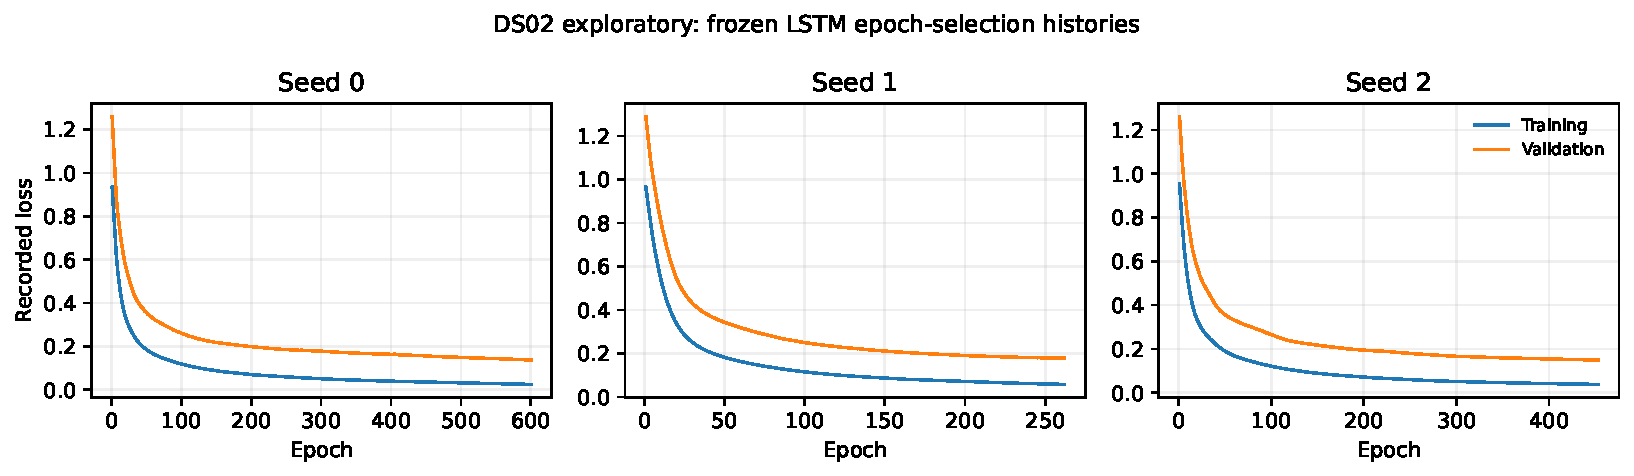
\includegraphics[width=0.9\textwidth]{../../submission/supplementary/figure_s1_ds02_lstm_history.pdf}
\caption{Frozen DS02 LSTM training and epoch-selection validation losses (seeds 0--2).}\label{fig:s1}
\end{figure}
\begin{figure}[htbp]\centering
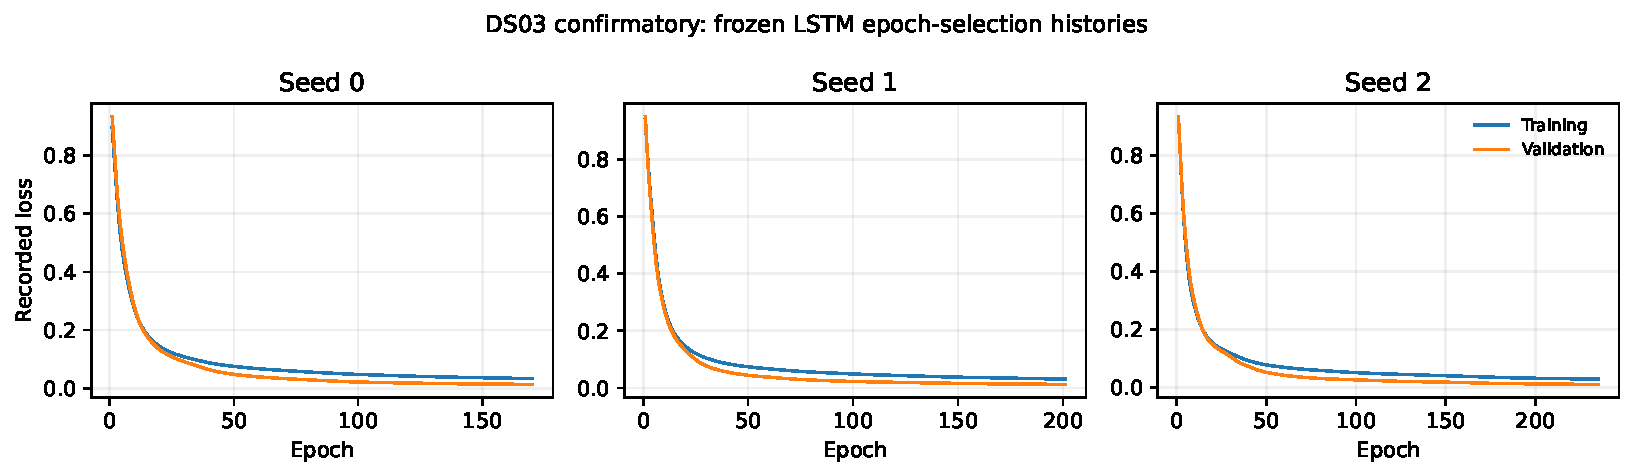
\includegraphics[width=0.9\textwidth]{../../submission/supplementary/figure_s2_ds03_lstm_history.pdf}
\caption{Frozen DS03 LSTM training and epoch-selection validation losses (seeds 0--2).}\label{fig:s2}
\end{figure}

\section{Post-confirmation protocol v1.0}
These analyses are exploratory. They reuse the frozen detectors and engine partitions and are not part of the
DS03 confirmation.

\begin{footnotesize}
\begin{longtable}{lllrrrr}
\caption{Post-confirmation pooled audit healthy FPR (\%) by phase at the 1\% target under P, C and C$'$ (protocol v1.0).}\label{tab:s8_phase_fpr}\\
\toprule
Dataset & Run & Arm & Climb & Cruise & Descent & Overall \\
\midrule
\endfirsthead
\multicolumn{7}{l}{\emph{(continued)}}\\
\toprule
Dataset & Run & Arm & Climb & Cruise & Descent & Overall \\
\midrule
\endhead
\bottomrule
\endfoot
DS02 & PCA & P & 0.125 & 0.428 & 3.459 & 1.363 \\
 &  & C & 1.403 & 1.327 & 1.081 & 1.265 \\
 &  & C$'$ & 1.462 & 1.075 & 1.360 & 1.273 \\
 & IF s0 & P & 0.285 & 0.566 & 2.335 & 1.084 \\
 &  & C & 1.655 & 1.845 & 0.921 & 1.485 \\
 &  & C$'$ & 1.525 & 1.119 & 1.669 & 1.410 \\
 & IF s1 & P & 0.253 & 0.528 & 2.669 & 1.172 \\
 &  & C & 1.544 & 1.528 & 0.978 & 1.348 \\
 &  & C$'$ & 1.434 & 1.099 & 1.699 & 1.389 \\
 & IF s2 & P & 0.266 & 0.580 & 2.455 & 1.125 \\
 &  & C & 1.686 & 1.715 & 0.927 & 1.443 \\
 &  & C$'$ & 1.560 & 1.125 & 1.680 & 1.426 \\
 & LSTM s0 & P & 0.452 & 0.707 & 2.078 & 1.099 \\
 &  & C & 1.385 & 1.115 & 1.080 & 1.175 \\
 &  & C$'$ & 1.377 & 1.541 & 1.778 & 1.577 \\
 & LSTM s1 & P & 0.474 & 0.731 & 2.102 & 1.122 \\
 &  & C & 1.243 & 1.279 & 0.961 & 1.163 \\
 &  & C$'$ & 1.200 & 1.390 & 1.725 & 1.452 \\
 & LSTM s2 & P & 0.539 & 0.750 & 2.060 & 1.133 \\
 &  & C & 1.456 & 1.073 & 1.001 & 1.150 \\
 &  & C$'$ & 1.419 & 1.503 & 1.748 & 1.563 \\
\midrule
DS03 & PCA & P & 0.877 & 0.912 & 1.977 & 1.341 \\
 &  & C & 1.856 & 1.789 & 1.231 & 1.577 \\
 &  & C$'$ & 1.977 & 1.108 & 1.685 & 1.564 \\
 & IF s0 & P & 0.417 & 1.095 & 2.166 & 1.364 \\
 &  & C & 1.656 & 1.394 & 1.271 & 1.410 \\
 &  & C$'$ & 1.053 & 0.827 & 1.694 & 1.240 \\
 & IF s1 & P & 0.399 & 1.060 & 2.127 & 1.332 \\
 &  & C & 1.663 & 1.366 & 1.267 & 1.400 \\
 &  & C$'$ & 1.037 & 0.791 & 1.672 & 1.215 \\
 & IF s2 & P & 0.412 & 1.157 & 2.134 & 1.370 \\
 &  & C & 1.745 & 1.424 & 1.268 & 1.441 \\
 &  & C$'$ & 1.083 & 0.882 & 1.719 & 1.276 \\
 & LSTM s0 & P & 0.759 & 1.795 & 2.231 & 1.713 \\
 &  & C & 1.777 & 1.830 & 1.488 & 1.676 \\
 &  & C$'$ & 1.841 & 1.833 & 1.723 & 1.790 \\
 & LSTM s1 & P & 0.719 & 1.890 & 2.220 & 1.730 \\
 &  & C & 1.845 & 1.756 & 1.495 & 1.671 \\
 &  & C$'$ & 1.879 & 1.931 & 1.625 & 1.792 \\
 & LSTM s2 & P & 0.774 & 1.982 & 2.193 & 1.764 \\
 &  & C & 1.796 & 1.720 & 1.529 & 1.661 \\
 &  & C$'$ & 1.877 & 2.004 & 1.746 & 1.866 \\
\end{longtable}
\end{footnotesize}

\begin{scriptsize}
\begin{longtable}{llllllll}
\caption{Paired arm-minus-P bootstrap 95\% intervals (percentage points) at the 1\% target for the row-pooled calibration metrics (frozen U1 resampling plans; engines then flights; thresholds re-estimated; 2000 replicates). A1, A2, A3 and A5 are row-pooled; the last column weights audit engines equally. Every interval includes zero.}\label{tab:s9_intervals}\\
\toprule
Dataset & Run & Arm $-$ P & A1 (pp) & A2 (pp) & A3 (pp) & A5 (pp) & \makecell{A2, equal-\\engine (pp)} \\
\midrule
\endfirsthead
\multicolumn{8}{l}{\emph{(continued)}}\\
\toprule
Dataset & Run & Arm $-$ P & A1 (pp) & A2 (pp) & A3 (pp) & A5 (pp) & \makecell{A2, equal-\\engine (pp)} \\
\midrule
\endhead
\bottomrule
\endfoot
DS02 & PCA & C & [$-$4.28, +0.63] & [$-$3.23, +1.21] & [$-$1.82, +0.85] & [$-$0.52, +1.21] & [$-$3.24, +2.90] \\
 &  & C$'$ & [$-$4.31, +1.49] & [$-$3.39, +2.83] & [$-$1.94, +1.77] & [$-$0.59, +1.74] & [$-$3.30, +5.81] \\
 & IF s0 & C & [$-$3.02, +4.92] & [$-$2.26, +4.34] & [$-$1.23, +3.03] & [$-$0.27, +1.86] & [$-$2.11, +5.41] \\
 &  & C$'$ & [$-$2.93, +3.06] & [$-$2.25, +3.92] & [$-$1.25, +2.80] & [$-$0.37, +1.99] & [$-$2.09, +5.04] \\
 & IF s1 & C & [$-$3.37, +3.92] & [$-$2.54, +3.23] & [$-$1.40, +2.36] & [$-$0.31, +1.26] & [$-$2.35, +4.52] \\
 &  & C$'$ & [$-$3.22, +2.06] & [$-$2.52, +3.22] & [$-$1.43, +2.35] & [$-$0.34, +1.69] & [$-$2.22, +4.24] \\
 & IF s2 & C & [$-$3.02, +5.30] & [$-$2.21, +4.51] & [$-$1.26, +3.25] & [$-$0.26, +1.77] & [$-$2.17, +5.94] \\
 &  & C$'$ & [$-$2.96, +3.31] & [$-$2.18, +4.28] & [$-$1.25, +2.89] & [$-$0.32, +1.97] & [$-$2.01, +5.69] \\
 & LSTM s0 & C & [$-$2.01, +3.89] & [$-$1.40, +3.65] & [$-$0.82, +2.13] & [$-$0.21, +1.25] & [$-$1.28, +5.65] \\
 &  & C$'$ & [$-$1.88, +2.31] & [$-$1.13, +3.38] & [$-$0.66, +2.47] & [$-$0.23, +2.20] & [$-$1.16, +5.32] \\
 & LSTM s1 & C & [$-$2.11, +3.18] & [$-$1.51, +2.66] & [$-$0.89, +1.66] & [$-$0.24, +1.03] & [$-$1.39, +3.37] \\
 &  & C$'$ & [$-$1.74, +1.86] & [$-$1.06, +2.49] & [$-$0.63, +2.09] & [$-$0.22, +1.86] & [$-$1.04, +3.11] \\
 & LSTM s2 & C & [$-$2.06, +4.03] & [$-$1.51, +3.67] & [$-$0.87, +2.16] & [$-$0.24, +1.01] & [$-$1.42, +5.95] \\
 &  & C$'$ & [$-$1.89, +2.62] & [$-$1.29, +3.35] & [$-$0.72, +2.56] & [$-$0.25, +2.17] & [$-$1.27, +5.51] \\
\midrule
DS03 & PCA & C & [$-$1.13, +2.56] & [$-$0.56, +2.61] & [$-$0.27, +1.51] & [$-$0.05, +0.92] & [$-$0.55, +2.43] \\
 &  & C$'$ & [$-$0.97, +2.91] & [$-$0.50, +3.67] & [$-$0.26, +2.21] & [$-$0.15, +1.48] & [$-$0.49, +3.61] \\
 & IF s0 & C & [$-$1.99, +4.43] & [$-$1.08, +4.85] & [$-$0.56, +2.68] & [$-$0.25, +1.34] & [$-$1.08, +5.00] \\
 &  & C$'$ & [$-$1.49, +1.82] & [$-$0.91, +2.49] & [$-$0.52, +1.39] & [$-$0.39, +0.99] & [$-$0.90, +2.51] \\
 & IF s1 & C & [$-$1.94, +4.25] & [$-$1.09, +4.70] & [$-$0.56, +2.63] & [$-$0.24, +1.35] & [$-$1.09, +4.69] \\
 &  & C$'$ & [$-$1.51, +1.71] & [$-$0.89, +2.46] & [$-$0.52, +1.40] & [$-$0.40, +1.01] & [$-$0.87, +2.42] \\
 & IF s2 & C & [$-$1.90, +4.88] & [$-$0.99, +5.27] & [$-$0.51, +2.96] & [$-$0.20, +1.44] & [$-$0.99, +5.47] \\
 &  & C$'$ & [$-$1.52, +2.12] & [$-$0.84, +2.85] & [$-$0.50, +1.65] & [$-$0.36, +1.11] & [$-$0.84, +2.84] \\
 & LSTM s0 & C & [$-$1.73, +1.82] & [$-$0.82, +1.97] & [$-$0.37, +1.08] & [$-$0.23, +0.45] & [$-$0.88, +2.45] \\
 &  & C$'$ & [$-$1.90, +1.08] & [$-$1.09, +1.65] & [$-$0.64, +0.97] & [$-$0.48, +0.77] & [$-$1.08, +2.04] \\
 & LSTM s1 & C & [$-$1.83, +1.84] & [$-$0.83, +1.89] & [$-$0.40, +1.01] & [$-$0.24, +0.43] & [$-$0.89, +2.35] \\
 &  & C$'$ & [$-$2.03, +1.11] & [$-$1.08, +1.52] & [$-$0.64, +0.91] & [$-$0.48, +0.68] & [$-$1.10, +1.92] \\
 & LSTM s2 & C & [$-$1.69, +2.52] & [$-$0.81, +2.48] & [$-$0.43, +1.38] & [$-$0.29, +0.59] & [$-$0.85, +3.05] \\
 &  & C$'$ & [$-$1.89, +1.57] & [$-$1.08, +2.07] & [$-$0.70, +1.18] & [$-$0.56, +0.92] & [$-$1.07, +2.49] \\
\end{longtable}
\end{scriptsize}

\begin{scriptsize}
\begin{longtable}{lp{0.5\textwidth}rrrl}
\caption{Target robustness of the post-confirmation claims: number of runs (of 7) in which each claim holds at the nominal targets 0.5\%, 1\% and 2\%, with the pre-specified classification.}\label{tab:s10_robustness}\\
\toprule
Dataset & Claim & 0.5\% & 1\% & 2\% & Class \\
\midrule
\endfirsthead
\multicolumn{6}{l}{\emph{(continued)}}\\
\toprule
Dataset & Claim & 0.5\% & 1\% & 2\% & Class \\
\midrule
\endhead
\bottomrule
\endfoot
DS02 & R1 descent is the highest pooled healthy-FPR phase (P) & 7/7 & 7/7 & 7/7 & invariant \\
 & R2 C reduces between-phase disparity (A1) & 7/7 & 7/7 & 7/7 & invariant \\
 & R3 C reduces max-abs nominal calibration error (A2) & 7/7 & 7/7 & 7/7 & invariant \\
 & R4 C reduces RMS nominal calibration error (A3) & 7/7 & 7/7 & 7/7 & invariant \\
 & R5 C mainly redistributes: |overall FPR change| $<$ 0.5 $\times$ |A1 change| & 6/7 & 7/7 & 7/7 & mostly invariant \\
 & R6 C abnormal-state row alarm-rate ratio $\geq$ 0.9 & 7/7 & 7/7 & 7/7 & invariant \\
 & R8 C is not earlier than P at matched false-flag burden & 4/7 & 4/7 & 3/7 & reversed \\
 & R2 C$'$ reduces between-phase disparity (A1) & 7/7 & 7/7 & 7/7 & invariant \\
 & R3 C$'$ reduces max-abs nominal calibration error (A2) & 4/7 & 7/7 & 7/7 & mostly invariant \\
 & R4 C$'$ reduces RMS nominal calibration error (A3) & 4/7 & 7/7 & 7/7 & mostly invariant \\
 & R5 C$'$ mainly redistributes: |overall FPR change| $<$ 0.5 $\times$ |A1 change| & 2/7 & 7/7 & 7/7 & reversed \\
 & R6 C$'$ abnormal-state row alarm-rate ratio $\geq$ 0.9 & 7/7 & 7/7 & 7/7 & invariant \\
 & R8 C$'$ is not earlier than P at matched false-flag burden & 7/7 & 3/7 & 2/7 & not supported at 1\% \\
 & R7 realized pooled healthy-flight FFR exceeds nominal 5\% (P) & 7/7 & 7/7 & 7/7 & invariant \\
 & R7 realized pooled healthy-flight FFR exceeds nominal 5\% (C) & 7/7 & 7/7 & 7/7 & invariant \\
 & R7 realized pooled healthy-flight FFR exceeds nominal 5\% (C$'$) & 7/7 & 7/7 & 7/7 & invariant \\
\midrule
DS03 & R1 descent is the highest pooled healthy-FPR phase (P) & 7/7 & 7/7 & 7/7 & invariant \\
 & R2 C reduces between-phase disparity (A1) & 7/7 & 7/7 & 7/7 & invariant \\
 & R3 C reduces max-abs nominal calibration error (A2) & 7/7 & 7/7 & 6/7 & mostly invariant \\
 & R4 C reduces RMS nominal calibration error (A3) & 7/7 & 6/7 & 6/7 & mostly invariant \\
 & R5 C mainly redistributes: |overall FPR change| $<$ 0.5 $\times$ |A1 change| & 7/7 & 7/7 & 7/7 & invariant \\
 & R6 C abnormal-state row alarm-rate ratio $\geq$ 0.9 & 7/7 & 7/7 & 7/7 & invariant \\
 & R8 C is not earlier than P at matched false-flag burden & 6/7 & 7/7 & 6/7 & mostly invariant \\
 & R2 C$'$ reduces between-phase disparity (A1) & 7/7 & 7/7 & 7/7 & invariant \\
 & R3 C$'$ reduces max-abs nominal calibration error (A2) & 6/7 & 7/7 & 6/7 & mostly invariant \\
 & R4 C$'$ reduces RMS nominal calibration error (A3) & 4/7 & 6/7 & 5/7 & target-sensitive \\
 & R5 C$'$ mainly redistributes: |overall FPR change| $<$ 0.5 $\times$ |A1 change| & 6/7 & 6/7 & 6/7 & mostly invariant \\
 & R6 C$'$ abnormal-state row alarm-rate ratio $\geq$ 0.9 & 7/7 & 7/7 & 7/7 & invariant \\
 & R8 C$'$ is not earlier than P at matched false-flag burden & 6/7 & 5/7 & 7/7 & mostly invariant \\
 & R7 realized pooled healthy-flight FFR exceeds nominal 5\% (P) & 7/7 & 6/7 & 7/7 & mostly invariant \\
 & R7 realized pooled healthy-flight FFR exceeds nominal 5\% (C) & 4/7 & 4/7 & 7/7 & target-sensitive \\
 & R7 realized pooled healthy-flight FFR exceeds nominal 5\% (C$'$) & 7/7 & 7/7 & 7/7 & invariant \\
\end{longtable}
\end{scriptsize}


\section{Adversarial validation}\label{sec:adversarial}
\begin{scriptsize}
\begin{longtable}{lllrrrr}
\caption{Per-engine maximum nominal calibration error A2 (percentage points) at the 1\% target for every detector run under P, C, C$'$ and Q.}\label{tab:s11_per_engine}\\
\toprule
Dataset & Engine (class) & Run & P & C & C$'$ & Q \\
\midrule
\endfirsthead
\multicolumn{7}{l}{\emph{(continued)}}\\
\toprule
Dataset & Engine (class) & Run & P & C & C$'$ & Q \\
\midrule
\endhead
\bottomrule
\endfoot
DS02 & 11 (3) & PCA & 1.78 & 0.38 & 0.63 & 2.00 \\
 &  & IF s0 & 1.23 & 0.25 & 0.97 & 1.45 \\
 &  & IF s1 & 1.35 & 0.35 & 0.99 & 1.28 \\
 &  & IF s2 & 1.30 & 0.25 & 0.97 & 1.48 \\
 &  & LSTM s0 & 1.36 & 0.36 & 1.11 & 0.61 \\
 &  & LSTM s1 & 1.52 & 0.38 & 1.15 & 0.44 \\
 &  & LSTM s2 & 1.38 & 0.36 & 1.07 & 4.25 \\
 & 14 (1) & PCA & 3.97 & 4.31 & 5.31 & 2.20 \\
 &  & IF s0 & 1.51 & 6.42 & 6.12 & 2.16 \\
 &  & IF s1 & 2.29 & 5.96 & 5.72 & 1.58 \\
 &  & IF s2 & 1.72 & 6.59 & 6.27 & 1.95 \\
 &  & LSTM s0 & 1.07 & 4.42 & 4.39 & 1.30 \\
 &  & LSTM s1 & 0.99 & 3.74 & 3.67 & 0.54 \\
 &  & LSTM s2 & 1.30 & 4.65 & 4.50 & 1.39 \\
 & 15 (2) & PCA & 2.67 & 0.28 & 0.40 & 0.58 \\
 &  & IF s0 & 1.40 & 0.27 & 0.57 & 3.63 \\
 &  & IF s1 & 1.82 & 0.26 & 0.56 & 1.08 \\
 &  & IF s2 & 1.55 & 0.28 & 0.55 & 4.15 \\
 &  & LSTM s0 & 0.66 & 0.19 & 0.23 & 0.62 \\
 &  & LSTM s1 & 0.66 & 0.14 & 0.29 & 0.64 \\
 &  & LSTM s2 & 0.71 & 0.30 & 0.27 & 4.18 \\
\midrule
DS03 & 10 (3) & PCA & 1.45 & 1.52 & 1.77 & 7.57 \\
 &  & IF s0 & 2.11 & 2.37 & 1.30 & 6.31 \\
 &  & IF s1 & 2.16 & 2.06 & 1.36 & 6.27 \\
 &  & IF s2 & 2.23 & 2.56 & 1.33 & 6.44 \\
 &  & LSTM s0 & 2.70 & 1.56 & 1.93 & 3.67 \\
 &  & LSTM s1 & 2.91 & 1.57 & 2.21 & 4.91 \\
 &  & LSTM s2 & 3.08 & 1.69 & 2.39 & 3.59 \\
 & 11 (3) & PCA & 1.17 & 0.97 & 1.14 & 0.56 \\
 &  & IF s0 & 1.28 & 0.52 & 0.93 & 0.89 \\
 &  & IF s1 & 1.32 & 0.49 & 0.93 & 0.87 \\
 &  & IF s2 & 1.29 & 0.50 & 0.96 & 0.89 \\
 &  & LSTM s0 & 1.67 & 0.99 & 1.16 & 0.84 \\
 &  & LSTM s1 & 1.62 & 0.91 & 1.02 & 0.81 \\
 &  & LSTM s2 & 1.65 & 0.97 & 1.16 & 0.76 \\
 & 12 (1) & PCA & 0.68 & 0.82 & 0.73 & 0.69 \\
 &  & IF s0 & 0.85 & 1.07 & 0.75 & 0.40 \\
 &  & IF s1 & 0.70 & 0.92 & 0.70 & 0.49 \\
 &  & IF s2 & 0.69 & 0.96 & 0.77 & 0.50 \\
 &  & LSTM s0 & 0.41 & 2.04 & 2.24 & 0.72 \\
 &  & LSTM s1 & 0.39 & 2.17 & 2.47 & 0.70 \\
 &  & LSTM s2 & 0.51 & 2.02 & 2.39 & 0.74 \\
 & 13 (3) & PCA & 1.25 & 1.22 & 1.42 & 1.41 \\
 &  & IF s0 & 1.66 & 0.77 & 0.77 & 1.69 \\
 &  & IF s1 & 1.60 & 0.86 & 0.75 & 1.24 \\
 &  & IF s2 & 1.62 & 0.81 & 0.80 & 1.33 \\
 &  & LSTM s0 & 1.69 & 1.47 & 1.10 & 0.64 \\
 &  & LSTM s1 & 1.67 & 1.22 & 1.20 & 0.70 \\
 &  & LSTM s2 & 1.81 & 1.39 & 1.21 & 0.58 \\
 & 14 (1) & PCA & 0.43 & 0.37 & 0.43 & 0.30 \\
 &  & IF s0 & 0.71 & 0.44 & 0.50 & 0.94 \\
 &  & IF s1 & 0.72 & 0.44 & 0.44 & 0.95 \\
 &  & IF s2 & 0.74 & 0.47 & 0.45 & 0.97 \\
 &  & LSTM s0 & 0.31 & 0.64 & 0.74 & 0.73 \\
 &  & LSTM s1 & 0.32 & 0.76 & 0.84 & 0.66 \\
 &  & LSTM s2 & 0.35 & 0.63 & 0.79 & 0.78 \\
 & 15 (2) & PCA & 1.15 & 1.28 & 1.20 & 0.54 \\
 &  & IF s0 & 0.62 & 0.25 & 0.34 & 0.65 \\
 &  & IF s1 & 0.64 & 0.40 & 0.35 & 0.62 \\
 &  & IF s2 & 0.63 & 0.38 & 0.43 & 0.66 \\
 &  & LSTM s0 & 0.56 & 0.65 & 0.69 & 0.50 \\
 &  & LSTM s1 & 0.45 & 0.54 & 0.54 & 0.49 \\
 &  & LSTM s2 & 0.38 & 0.74 & 0.83 & 0.61 \\
\end{longtable}
\end{scriptsize}

\begin{scriptsize}
\begin{longtable}{lp{0.62\textwidth}r}
\caption{Denominator audit: sign agreement between row-pooled and alternative weightings or endpoints, over runs, targets and arms. The frozen burden endpoint (healthy flights with any alarm) and the $\kappa$-based healthy-flight false-flag rate are distinct quantities.}\label{tab:s12_weighting}\\
\toprule
Dataset & Check & Agreeing \\
\midrule
\endfirsthead
\multicolumn{3}{l}{\emph{(continued)}}\\
\toprule
Dataset & Check & Agreeing \\
\midrule
\endhead
\bottomrule
\endfoot
DS02 & row-pooled vs equal-engine sign of diff\_spread & 25 of 42 \\
 & row-pooled vs equal-engine sign of diff\_max\_abs\_error & 16 of 42 \\
 & row-pooled vs equal-engine sign of diff\_rms\_error & 15 of 42 \\
 & equal-flight vs row-pooled sign of overall healthy FPR change (phase\_conditioned) & 19 of 21 \\
 & equal-flight vs row-pooled sign of overall healthy FPR change (causal\_regime) & 19 of 21 \\
 & `healthy flights with any alarm` vs kappa FFR sign of change (phase\_conditioned) & 8 of 21 \\
 & `healthy flights with any alarm` vs kappa FFR sign of change (causal\_regime) & 8 of 21 \\
 & row abnormal alarm rate higher vs flight delay earlier (phase\_conditioned) & 5 of 21 \\
 & row abnormal alarm rate higher vs flight delay earlier (causal\_regime) & 13 of 21 \\
\midrule
DS03 & row-pooled vs equal-engine sign of diff\_spread & 42 of 42 \\
 & row-pooled vs equal-engine sign of diff\_max\_abs\_error & 39 of 42 \\
 & row-pooled vs equal-engine sign of diff\_rms\_error & 36 of 42 \\
 & equal-flight vs row-pooled sign of overall healthy FPR change (phase\_conditioned) & 14 of 21 \\
 & equal-flight vs row-pooled sign of overall healthy FPR change (causal\_regime) & 19 of 21 \\
 & `healthy flights with any alarm` vs kappa FFR sign of change (phase\_conditioned) & 0 of 21 \\
 & `healthy flights with any alarm` vs kappa FFR sign of change (causal\_regime) & 4 of 21 \\
 & row abnormal alarm rate higher vs flight delay earlier (phase\_conditioned) & 10 of 21 \\
 & row abnormal alarm rate higher vs flight delay earlier (causal\_regime) & 13 of 21 \\
\end{longtable}
\end{scriptsize}


\subsection*{Matched false-flag delay}
Figure~\ref{fig:s3} shows the full operating characteristics: the lower-median detection delay against the realized
pooled healthy-flight false-flag rate as $\kappa$ is swept over the calibration-only grid. Tables~\ref{tab:s13_matched}
and~\ref{tab:s14_labels} give the matched comparisons at the pre-specified anchors, and Table~\ref{tab:s15_delays}
gives per-engine delays at the locked $\kappa$ together with their false-flag rates.

\begin{figure}[htbp]\centering
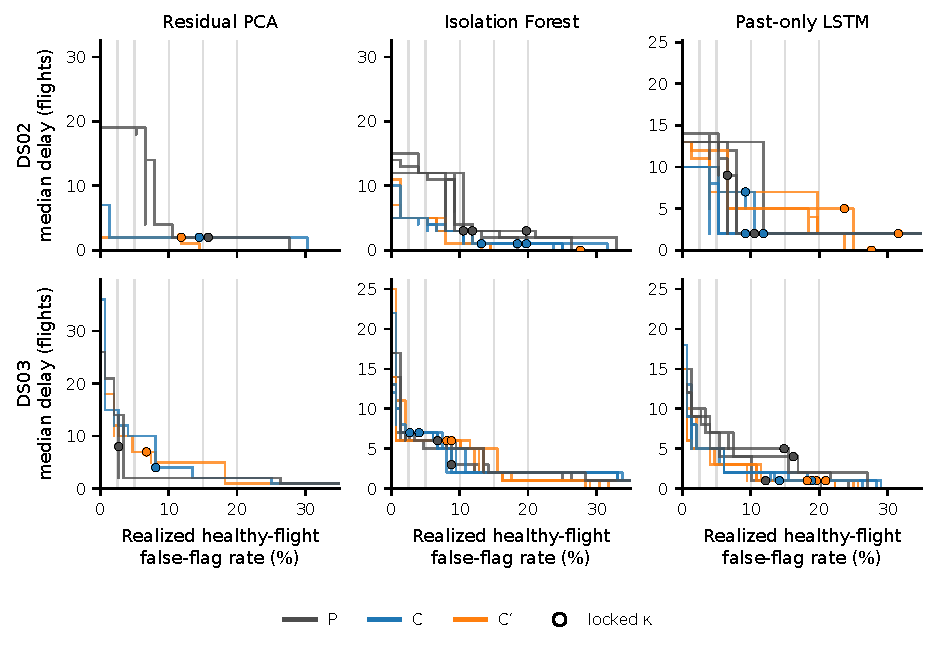
\includegraphics[width=\textwidth]{figures/figS3_operating_characteristics.pdf}
\caption{Median detection delay against realized pooled healthy-flight false-flag rate at the 1\% row target, one step
curve per seed and arm over the calibration-only $\kappa$ grid. Grey vertical lines mark the matching anchors; filled
markers are the locked-$\kappa$ operating points (nominal 5\%). Vertical segments mark $\kappa$ intervals that share a
realized rate.}\label{fig:s3}
\end{figure}

\begin{scriptsize}
\begin{longtable}{lllrlllll}
\caption{Matched healthy-flight false-flag comparisons at the 1\% row target (nearest-anchor rule): realized pooled false-flag rates, lower-median delays (flights from the labelled abnormal-state onset), per-engine earlier/same/later counts, and the paired lower-median difference (arm $-$ P). Unsupported anchors are shown but were not used.}\label{tab:s13_matched}\\
\toprule
Dataset & Run & Arm & \makecell{Anchor\\(\%)} & \makecell{Sup-\\ported} & \makecell{FFR (\%)\\P / arm} & \makecell{Median delay\\P / arm} & \makecell{Engines earlier/\\same/later} & \makecell{Paired\\median diff.} \\
\midrule
\endfirsthead
\multicolumn{9}{l}{\emph{(continued)}}\\
\toprule
Dataset & Run & Arm & \makecell{Anchor\\(\%)} & \makecell{Sup-\\ported} & \makecell{FFR (\%)\\P / arm} & \makecell{Median delay\\P / arm} & \makecell{Engines earlier/\\same/later} & \makecell{Paired\\median diff.} \\
\midrule
\endhead
\bottomrule
\endfoot
DS02 & PCA & C & 2.5 & yes & 2.6 / 2.6 & 19 / 2 & 3/0/0 & $-$13 \\
 &  & C & 5 & yes & 5.3 / 5.3 & 19 / 2 & 3/0/0 & $-$13 \\
 &  & C & 10 & no & 10.5 / 11.8 & 4 / 2 & 1/1/1 & 0 \\
 &  & C & 15 & yes & 14.5 / 14.5 & 2 / 2 & 1/1/1 & 0 \\
 &  & C & 20 & yes & 19.7 / 19.7 & 2 / 2 & 1/1/1 & 0 \\
 &  & C$'$ & 2.5 & yes & 2.6 / 1.3 & 19 / 2 & 3/0/0 & $-$13 \\
 &  & C$'$ & 5 & yes & 5.3 / 5.3 & 19 / 2 & 3/0/0 & $-$13 \\
 &  & C$'$ & 10 & yes & 10.5 / 10.5 & 4 / 2 & 1/1/1 & 0 \\
 &  & C$'$ & 15 & yes & 14.5 / 14.5 & 2 / 1 & 2/0/1 & $-$2 \\
 &  & C$'$ & 20 & no & 19.7 / 18.4 & 2 / 0 & 2/0/1 & $-$2 \\
 & IF s0 & C & 2.5 & yes & 2.6 / 1.3 & 12 / 5 & 3/0/0 & $-$7 \\
 &  & C & 5 & yes & 5.3 / 5.3 & 11 / 5 & 3/0/0 & $-$6 \\
 &  & C & 10 & yes & 10.5 / 10.5 & 4 / 3 & 2/1/0 & $-$3 \\
 &  & C & 15 & yes & 15.8 / 14.5 & 2 / 1 & 1/2/0 & 0 \\
 &  & C & 20 & no & 18.4 / 19.7 & 2 / 1 & 1/0/2 & 1 \\
 &  & C$'$ & 2.5 & yes & 2.6 / 1.3 & 12 / 5 & 3/0/0 & $-$7 \\
 &  & C$'$ & 5 & yes & 5.3 / 5.3 & 11 / 5 & 3/0/0 & $-$6 \\
 &  & C$'$ & 10 & yes & 10.5 / 10.5 & 4 / 3 & 2/1/0 & $-$3 \\
 &  & C$'$ & 15 & yes & 15.8 / 14.5 & 2 / 0 & 2/1/0 & $-$1 \\
 &  & C$'$ & 20 & no & 18.4 / 19.7 & 2 / 0 & 1/1/1 & 0 \\
 & IF s1 & C & 2.5 & yes & 1.3 / 1.3 & 15 / 5 & 3/0/0 & $-$7 \\
 &  & C & 5 & yes & 5.3 / 5.3 & 12 / 5 & 3/0/0 & $-$7 \\
 &  & C & 10 & yes & 10.5 / 10.5 & 6 / 3 & 2/1/0 & $-$5 \\
 &  & C & 15 & yes & 14.5 / 14.5 & 3 / 1 & 2/1/0 & $-$2 \\
 &  & C & 20 & yes & 19.7 / 19.7 & 3 / 1 & 2/1/0 & $-$2 \\
 &  & C$'$ & 2.5 & yes & 1.3 / 1.3 & 15 / 5 & 3/0/0 & $-$8 \\
 &  & C$'$ & 5 & yes & 5.3 / 5.3 & 12 / 5 & 3/0/0 & $-$7 \\
 &  & C$'$ & 10 & yes & 10.5 / 10.5 & 6 / 3 & 2/1/0 & $-$5 \\
 &  & C$'$ & 15 & yes & 14.5 / 15.8 & 3 / 0 & 2/1/0 & $-$2 \\
 &  & C$'$ & 20 & yes & 19.7 / 19.7 & 3 / 0 & 2/1/0 & $-$2 \\
 & IF s2 & C & 2.5 & yes & 2.6 / 1.3 & 13 / 5 & 3/0/0 & $-$7 \\
 &  & C & 5 & yes & 5.3 / 5.3 & 12 / 4 & 3/0/0 & $-$7 \\
 &  & C & 10 & yes & 10.5 / 10.5 & 3 / 3 & 1/1/1 & 0 \\
 &  & C & 15 & yes & 14.5 / 14.5 & 2 / 1 & 2/0/1 & $-$1 \\
 &  & C & 20 & yes & 19.7 / 19.7 & 0 / 1 & 1/1/1 & 0 \\
 &  & C$'$ & 2.5 & yes & 2.6 / 1.3 & 13 / 5 & 3/0/0 & $-$7 \\
 &  & C$'$ & 5 & yes & 5.3 / 5.3 & 12 / 5 & 3/0/0 & $-$7 \\
 &  & C$'$ & 10 & yes & 10.5 / 10.5 & 3 / 1 & 2/1/0 & $-$2 \\
 &  & C$'$ & 15 & yes & 14.5 / 14.5 & 2 / 0 & 2/0/1 & $-$2 \\
 &  & C$'$ & 20 & yes & 19.7 / 19.7 & 0 / 0 & 0/2/1 & 0 \\
 & LSTM s0 & C & 2.5 & no & 3.9 / 1.3 & 14 / 10 & 3/0/0 & $-$4 \\
 &  & C & 5 & yes & 5.3 / 5.3 & 13 / 5 & 3/0/0 & $-$8 \\
 &  & C & 10 & no & 11.8 / 10.5 & 11 / 2 & 2/0/1 & $-$4 \\
 &  & C & 15 & yes & 14.5 / 14.5 & 2 / 2 & 0/2/1 & 0 \\
 &  & C & 20 & yes & 19.7 / 21.1 & 2 / 2 & 0/2/1 & 0 \\
 &  & C$'$ & 2.5 & no & 3.9 / 1.3 & 14 / 11 & 3/0/0 & $-$3 \\
 &  & C$'$ & 5 & yes & 5.3 / 5.3 & 13 / 7 & 3/0/0 & $-$6 \\
 &  & C$'$ & 10 & no & 11.8 / 10.5 & 11 / 5 & 2/0/1 & $-$3 \\
 &  & C$'$ & 15 & yes & 14.5 / 14.5 & 2 / 5 & 0/1/2 & 3 \\
 &  & C$'$ & 20 & yes & 19.7 / 19.7 & 2 / 5 & 0/1/2 & 3 \\
 & LSTM s1 & C & 2.5 & yes & 1.3 / 2.6 & 13 / 10 & 3/0/0 & $-$6 \\
 &  & C & 5 & yes & 5.3 / 5.3 & 13 / 7 & 3/0/0 & $-$5 \\
 &  & C & 10 & yes & 10.5 / 10.5 & 2 / 5 & 1/0/2 & 1 \\
 &  & C & 15 & yes & 14.5 / 14.5 & 2 / 2 & 0/1/2 & 1 \\
 &  & C & 20 & yes & 19.7 / 21.1 & 2 / 2 & 0/2/1 & 0 \\
 &  & C$'$ & 2.5 & yes & 1.3 / 1.3 & 13 / 10 & 3/0/0 & $-$4 \\
 &  & C$'$ & 5 & yes & 5.3 / 5.3 & 13 / 7 & 3/0/0 & $-$6 \\
 &  & C$'$ & 10 & yes & 10.5 / 10.5 & 2 / 7 & 1/0/2 & 1 \\
 &  & C$'$ & 15 & yes & 14.5 / 14.5 & 2 / 7 & 0/1/2 & 5 \\
 &  & C$'$ & 20 & yes & 19.7 / 19.7 & 2 / 7 & 0/1/2 & 5 \\
 & LSTM s2 & C & 2.5 & no & 3.9 / 2.6 & 13 / 10 & 2/1/0 & $-$4 \\
 &  & C & 5 & yes & 5.3 / 5.3 & 11 / 2 & 3/0/0 & $-$8 \\
 &  & C & 10 & no & 7.9 / 9.2 & 2 / 2 & 1/1/1 & 0 \\
 &  & C & 15 & yes & 14.5 / 14.5 & 2 / 2 & 0/2/1 & 0 \\
 &  & C & 20 & yes & 21.1 / 21.1 & 2 / 2 & 0/2/1 & 0 \\
 &  & C$'$ & 2.5 & no & 3.9 / 2.6 & 13 / 12 & 3/0/0 & $-$2 \\
 &  & C$'$ & 5 & yes & 5.3 / 3.9 & 11 / 12 & 1/1/1 & 0 \\
 &  & C$'$ & 10 & no & 7.9 / 10.5 & 2 / 5 & 1/0/2 & 1 \\
 &  & C$'$ & 15 & yes & 14.5 / 14.5 & 2 / 5 & 0/1/2 & 3 \\
 &  & C$'$ & 20 & yes & 21.1 / 19.7 & 2 / 2 & 0/2/1 & 0 \\
\midrule
DS03 & PCA & C & 2.5 & yes & 2.7 / 2.7 & 14 / 12 & 3/0/3 & $-$4 \\
 &  & C & 5 & no & 4.1 / 4.7 & 2 / 10 & 3/0/3 & $-$5 \\
 &  & C & 10 & yes & 10.1 / 10.1 & 2 / 4 & 1/2/3 & 0 \\
 &  & C & 15 & no & 14.2 / 15.5 & 2 / 2 & 1/4/1 & 0 \\
 &  & C & 20 & yes & 19.6 / 20.3 & 2 / 2 & 1/3/2 & 0 \\
 &  & C$'$ & 2.5 & yes & 2.7 / 2.7 & 14 / 10 & 3/0/3 & $-$4 \\
 &  & C$'$ & 5 & no & 4.1 / 4.7 & 2 / 10 & 3/0/3 & $-$4 \\
 &  & C$'$ & 10 & yes & 10.1 / 10.1 & 2 / 5 & 1/0/5 & 1 \\
 &  & C$'$ & 15 & no & 14.2 / 15.5 & 2 / 5 & 2/0/4 & 1 \\
 &  & C$'$ & 20 & yes & 19.6 / 19.6 & 2 / 1 & 2/1/3 & 0 \\
 & IF s0 & C & 2.5 & yes & 2.7 / 2.0 & 6 / 7 & 0/2/4 & 1 \\
 &  & C & 5 & yes & 4.7 / 4.7 & 5 / 7 & 0/2/4 & 1 \\
 &  & C & 10 & yes & 10.1 / 10.1 & 3 / 2 & 2/2/2 & 0 \\
 &  & C & 15 & yes & 15.5 / 15.5 & 2 / 2 & 1/3/2 & 0 \\
 &  & C & 20 & yes & 20.3 / 20.3 & 2 / 2 & 1/4/1 & 0 \\
 &  & C$'$ & 2.5 & yes & 2.7 / 2.7 & 6 / 6 & 2/4/0 & 0 \\
 &  & C$'$ & 5 & yes & 4.7 / 5.4 & 5 / 6 & 2/3/1 & 0 \\
 &  & C$'$ & 10 & yes & 10.1 / 10.1 & 3 / 5 & 3/1/2 & $-$3 \\
 &  & C$'$ & 15 & no & 15.5 / 16.2 & 2 / 1 & 1/3/2 & 0 \\
 &  & C$'$ & 20 & yes & 20.3 / 20.3 & 2 / 1 & 1/3/2 & 0 \\
 & IF s1 & C & 2.5 & yes & 2.7 / 2.0 & 6 / 7 & 1/3/2 & 0 \\
 &  & C & 5 & yes & 4.7 / 4.7 & 6 / 7 & 0/4/2 & 0 \\
 &  & C & 10 & no & 9.5 / 8.8 & 6 / 2 & 3/3/0 & $-$1 \\
 &  & C & 15 & yes & 14.9 / 14.9 & 2 / 2 & 1/4/1 & 0 \\
 &  & C & 20 & yes & 20.3 / 20.3 & 2 / 2 & 1/4/1 & 0 \\
 &  & C$'$ & 2.5 & yes & 2.7 / 2.0 & 6 / 6 & 1/5/0 & 0 \\
 &  & C$'$ & 5 & yes & 4.7 / 5.4 & 6 / 6 & 1/5/0 & 0 \\
 &  & C$'$ & 10 & yes & 9.5 / 10.1 & 6 / 6 & 2/3/1 & 0 \\
 &  & C$'$ & 15 & yes & 14.9 / 14.9 & 2 / 2 & 1/3/2 & 0 \\
 &  & C$'$ & 20 & yes & 20.3 / 20.3 & 2 / 1 & 1/3/2 & 0 \\
 & IF s2 & C & 2.5 & yes & 2.0 / 2.7 & 7 / 7 & 2/2/2 & 0 \\
 &  & C & 5 & yes & 5.4 / 4.7 & 6 / 7 & 1/3/2 & 0 \\
 &  & C & 10 & yes & 9.5 / 9.5 & 5 / 5 & 2/1/3 & 0 \\
 &  & C & 15 & no & 15.5 / 14.2 & 2 / 2 & 1/4/1 & 0 \\
 &  & C & 20 & no & 20.3 / 18.9 & 2 / 2 & 1/4/1 & 0 \\
 &  & C$'$ & 2.5 & yes & 2.0 / 2.0 & 7 / 6 & 5/1/0 & $-$3 \\
 &  & C$'$ & 5 & yes & 5.4 / 4.7 & 6 / 6 & 2/4/0 & 0 \\
 &  & C$'$ & 10 & yes & 9.5 / 10.1 & 5 / 6 & 3/1/2 & $-$1 \\
 &  & C$'$ & 15 & yes & 15.5 / 15.5 & 2 / 2 & 1/2/3 & 0 \\
 &  & C$'$ & 20 & yes & 20.3 / 20.3 & 2 / 1 & 1/3/2 & 0 \\
 & LSTM s0 & C & 2.5 & yes & 2.7 / 2.7 & 10 / 5 & 4/2/0 & $-$8 \\
 &  & C & 5 & yes & 4.7 / 4.7 & 7 / 5 & 3/2/1 & $-$2 \\
 &  & C & 10 & yes & 10.1 / 10.1 & 4 / 2 & 2/3/1 & 0 \\
 &  & C & 15 & yes & 14.9 / 14.9 & 4 / 2 & 2/2/2 & 0 \\
 &  & C & 20 & yes & 20.3 / 19.6 & 2 / 1 & 1/3/2 & 0 \\
 &  & C$'$ & 2.5 & yes & 2.7 / 2.0 & 10 / 5 & 4/1/1 & $-$3 \\
 &  & C$'$ & 5 & yes & 4.7 / 4.7 & 7 / 3 & 5/0/1 & $-$8 \\
 &  & C$'$ & 10 & yes & 10.1 / 9.5 & 4 / 3 & 4/1/1 & $-$1 \\
 &  & C$'$ & 15 & yes & 14.9 / 14.9 & 4 / 1 & 3/3/0 & $-$1 \\
 &  & C$'$ & 20 & yes & 20.3 / 20.3 & 2 / 1 & 3/2/1 & $-$1 \\
 & LSTM s1 & C & 2.5 & yes & 2.7 / 2.7 & 8 / 5 & 4/2/0 & $-$4 \\
 &  & C & 5 & yes & 4.7 / 5.4 & 7 / 5 & 4/2/0 & $-$3 \\
 &  & C & 10 & yes & 10.1 / 9.5 & 1 / 2 & 1/2/3 & 0 \\
 &  & C & 15 & yes & 14.9 / 15.5 & 1 / 1 & 1/2/3 & 0 \\
 &  & C & 20 & yes & 20.3 / 19.6 & 1 / 1 & 1/3/2 & 0 \\
 &  & C$'$ & 2.5 & yes & 2.7 / 2.7 & 8 / 5 & 5/0/1 & $-$4 \\
 &  & C$'$ & 5 & yes & 4.7 / 5.4 & 7 / 5 & 4/0/2 & $-$4 \\
 &  & C$'$ & 10 & yes & 10.1 / 9.5 & 1 / 3 & 1/4/1 & 0 \\
 &  & C$'$ & 15 & yes & 14.9 / 15.5 & 1 / 1 & 1/3/2 & 0 \\
 &  & C$'$ & 20 & yes & 20.3 / 20.3 & 1 / 1 & 1/3/2 & 0 \\
 & LSTM s2 & C & 2.5 & yes & 2.7 / 2.0 & 9 / 5 & 4/1/1 & $-$4 \\
 &  & C & 5 & yes & 4.7 / 4.7 & 5 / 5 & 3/2/1 & $-$4 \\
 &  & C & 10 & yes & 10.1 / 9.5 & 5 / 2 & 2/2/2 & 0 \\
 &  & C & 15 & yes & 14.9 / 14.9 & 5 / 1 & 2/3/1 & 0 \\
 &  & C & 20 & yes & 20.3 / 20.3 & 2 / 1 & 2/2/2 & 0 \\
 &  & C$'$ & 2.5 & yes & 2.7 / 2.7 & 9 / 5 & 5/0/1 & $-$4 \\
 &  & C$'$ & 5 & yes & 4.7 / 4.7 & 5 / 3 & 4/1/1 & $-$4 \\
 &  & C$'$ & 10 & yes & 10.1 / 9.5 & 5 / 3 & 2/3/1 & 0 \\
 &  & C$'$ & 15 & no & 14.9 / 14.2 & 5 / 1 & 2/4/0 & 0 \\
 &  & C$'$ & 20 & no & 20.3 / 18.9 & 2 / 1 & 2/2/2 & 0 \\
\end{longtable}
\end{scriptsize}

\begin{scriptsize}
\begin{longtable}{lllrllll}
\caption{Pre-specified run labels at the 1\% target under the nearest-anchor rule and the conservative (not-exceeding) sensitivity rule, curve-level mean delays over realized false-flag rates 2.5--20\% (flights), and the Pareto class of the locked operating point against P. Labels: E, earlier at matched burden; L, later; M, mixed; =, equal; n/e, not evaluable.}\label{tab:s14_labels}\\
\toprule
Dataset & Run & Arm & \makecell{Supported\\anchors} & \makecell{Label\\(nearest)} & \makecell{Label\\(conservative)} & \makecell{Curve mean\\P / arm} & \makecell{Locked\\point} \\
\midrule
\endfirsthead
\multicolumn{8}{l}{\emph{(continued)}}\\
\toprule
Dataset & Run & Arm & \makecell{Supported\\anchors} & \makecell{Label\\(nearest)} & \makecell{Label\\(conservative)} & \makecell{Curve mean\\P / arm} & \makecell{Locked\\point} \\
\midrule
\endhead
\bottomrule
\endfoot
DS02 & PCA & C & 4 & M & M & 6.93 / 2.00 & arm dominates \\
 & IF s0 & C & 4 & E & E & 6.09 / 2.38 & trade-off \\
 & IF s1 & C & 5 & E & E & 7.17 / 2.38 & arm dominates \\
 & IF s2 & C & 5 & E & E & 5.75 / 2.38 & trade-off \\
 & LSTM s0 & C & 3 & M & M & 6.74 / 3.23 & identical \\
 & LSTM s1 & C & 5 & M & M & 4.87 / 4.91 & trade-off \\
 & LSTM s2 & C & 3 & M & M & 4.85 / 3.01 & trade-off \\
 & PCA & C$'$ & 4 & E & E & 6.93 / 1.52 & arm dominates \\
 & IF s0 & C$'$ & 4 & E & E & 6.09 / 2.33 & trade-off \\
 & IF s1 & C$'$ & 5 & E & E & 7.17 / 2.27 & trade-off \\
 & IF s2 & C$'$ & 5 & E & E & 5.75 / 1.58 & trade-off \\
 & LSTM s0 & C$'$ & 3 & M & M & 6.74 / 5.97 & arm dominated \\
 & LSTM s1 & C$'$ & 5 & M & M & 4.87 / 7.41 & arm dominated \\
 & LSTM s2 & C$'$ & 3 & M & M & 4.85 / 6.09 & trade-off \\
\midrule
DS03 & PCA & C & 3 & M & E & 2.61 / 5.70 & trade-off \\
 & IF s0 & C & 5 & M & M & 3.54 / 3.28 & trade-off \\
 & IF s1 & C & 4 & = & = & 4.09 / 3.96 & trade-off \\
 & IF s2 & C & 3 & = & = & 4.53 / 3.84 & trade-off \\
 & LSTM s0 & C & 5 & M & M & 4.83 / 2.26 & trade-off \\
 & LSTM s1 & C & 5 & M & = & 3.00 / 2.31 & arm dominated \\
 & LSTM s2 & C & 5 & M & E & 4.72 / 2.42 & arm dominates \\
 & PCA & C$'$ & 3 & M & M & 2.61 / 5.59 & trade-off \\
 & IF s0 & C$'$ & 4 & M & M & 3.54 / 3.94 & arm dominated \\
 & IF s1 & C$'$ & 5 & = & M & 4.09 / 3.96 & arm dominates \\
 & IF s2 & C$'$ & 5 & M & E & 4.53 / 4.23 & arm dominated \\
 & LSTM s0 & C$'$ & 5 & E & E & 4.83 / 2.25 & trade-off \\
 & LSTM s1 & C$'$ & 5 & M & = & 3.00 / 2.24 & arm dominated \\
 & LSTM s2 & C$'$ & 3 & E & E & 4.72 / 2.12 & trade-off \\
\end{longtable}
\end{scriptsize}

\begin{scriptsize}
\begin{longtable}{lllrll}
\caption{Per-engine detection delay (flights from the labelled abnormal-state onset; cens. = no flagged post-onset flight) and healthy-flight false-flag rate at the locked $\kappa$ (1\% row target).}\label{tab:s15_delays}\\
\toprule
Dataset & Run & Engine & P: delay / FFR (\%) & C: delay / FFR (\%) & C$'$: delay / FFR (\%) \\
\midrule
\endfirsthead
\multicolumn{6}{l}{\emph{(continued)}}\\
\toprule
Dataset & Run & Engine & P: delay / FFR (\%) & C: delay / FFR (\%) & C$'$: delay / FFR (\%) \\
\midrule
\endhead
\bottomrule
\endfoot
DS02 & PCA & 11 & 2 / 5.6 & 10 / 0.0 & 10 / 0.0 \\
 &  & 14 & 4 / 17.1 & 1 / 28.6 & 1 / 25.7 \\
 &  & 15 & 2 / 21.7 & 2 / 4.3 & 2 / 0.0 \\
 & IF s0 & 11 & 3 / 5.6 & 3 / 5.6 & 3 / 5.6 \\
 &  & 14 & 4 / 17.1 & 1 / 34.3 & 0 / 54.3 \\
 &  & 15 & 2 / 4.3 & 0 / 4.3 & 0 / 4.3 \\
 & IF s1 & 11 & 3 / 5.6 & 3 / 5.6 & 3 / 5.6 \\
 &  & 14 & 4 / 25.7 & 1 / 22.9 & 0 / 54.3 \\
 &  & 15 & 2 / 21.7 & 0 / 4.3 & 0 / 4.3 \\
 & IF s2 & 11 & 3 / 5.6 & 1 / 5.6 & 3 / 5.6 \\
 &  & 14 & 4 / 17.1 & 1 / 37.1 & 0 / 54.3 \\
 &  & 15 & 2 / 8.7 & 0 / 4.3 & 0 / 4.3 \\
 & LSTM s0 & 11 & 11 / 5.6 & 7 / 0.0 & 5 / 5.6 \\
 &  & 14 & 0 / 22.9 & 1 / 22.9 & 0 / 57.1 \\
 &  & 15 & 2 / 0.0 & 2 / 4.3 & 2 / 13.0 \\
 & LSTM s1 & 11 & 13 / 5.6 & 10 / 0.0 & 5 / 5.6 \\
 &  & 14 & 0 / 20.0 & 1 / 20.0 & 0 / 45.7 \\
 &  & 15 & 2 / 0.0 & 7 / 0.0 & 5 / 4.3 \\
 & LSTM s2 & 11 & 11 / 5.6 & 5 / 0.0 & 5 / 5.6 \\
 &  & 14 & 9 / 8.6 & 1 / 14.3 & 0 / 51.4 \\
 &  & 15 & 2 / 4.3 & 2 / 8.7 & 0 / 8.7 \\
\midrule
DS03 & PCA & 10 & 23 / 5.9 & 17 / 11.8 & 19 / 11.8 \\
 &  & 11 & 8 / 0.0 & 2 / 0.0 & 5 / 5.6 \\
 &  & 12 & 15 / 0.0 & 10 / 13.9 & 7 / 0.0 \\
 &  & 13 & 2 / 5.6 & 2 / 11.1 & 1 / 16.7 \\
 &  & 14 & 14 / 0.0 & 4 / 0.0 & 7 / 2.9 \\
 &  & 15 & 1 / 8.3 & 12 / 12.5 & 11 / 12.5 \\
 & IF s0 & 10 & 18 / 5.9 & 19 / 5.9 & 18 / 11.8 \\
 &  & 11 & 3 / 11.1 & 7 / 0.0 & 6 / 5.6 \\
 &  & 12 & 0 / 8.3 & 1 / 2.8 & 0 / 8.3 \\
 &  & 13 & 18 / 11.1 & 18 / 11.1 & 18 / 0.0 \\
 &  & 14 & 5 / 11.4 & 6 / 5.7 & 2 / 11.4 \\
 &  & 15 & 1 / 4.2 & 8 / 0.0 & 6 / 12.5 \\
 & IF s1 & 10 & 19 / 11.8 & 19 / 5.9 & 18 / 11.8 \\
 &  & 11 & 6 / 11.1 & 7 / 0.0 & 6 / 5.6 \\
 &  & 12 & 0 / 5.6 & 0 / 2.8 & 0 / 8.3 \\
 &  & 13 & 18 / 11.1 & 18 / 11.1 & 18 / 0.0 \\
 &  & 14 & 6 / 11.4 & 6 / 5.7 & 3 / 11.4 \\
 &  & 15 & 1 / 4.2 & 8 / 0.0 & 6 / 8.3 \\
 & IF s2 & 10 & 19 / 5.9 & 19 / 5.9 & 18 / 11.8 \\
 &  & 11 & 6 / 5.6 & 7 / 0.0 & 6 / 5.6 \\
 &  & 12 & 3 / 5.6 & 4 / 2.8 & 0 / 8.3 \\
 &  & 13 & 18 / 11.1 & 18 / 11.1 & 18 / 0.0 \\
 &  & 14 & 6 / 8.6 & 6 / 0.0 & 5 / 11.4 \\
 &  & 15 & 6 / 4.2 & 8 / 0.0 & 6 / 12.5 \\
 & LSTM s0 & 10 & 6 / 35.3 & 6 / 41.2 & 5 / 29.4 \\
 &  & 11 & 5 / 11.1 & 2 / 22.2 & 5 / 16.7 \\
 &  & 12 & 4 / 5.6 & 1 / 11.1 & 0 / 19.4 \\
 &  & 13 & 1 / 38.9 & 1 / 33.3 & 0 / 27.8 \\
 &  & 14 & 5 / 8.6 & 5 / 8.6 & 3 / 11.4 \\
 &  & 15 & 1 / 16.7 & 1 / 20.8 & 1 / 20.8 \\
 & LSTM s1 & 10 & 5 / 41.2 & 6 / 47.1 & 5 / 35.3 \\
 &  & 11 & 2 / 11.1 & 2 / 16.7 & 5 / 16.7 \\
 &  & 12 & 0 / 0.0 & 0 / 11.1 & 0 / 22.2 \\
 &  & 13 & 1 / 27.8 & 1 / 27.8 & 1 / 27.8 \\
 &  & 14 & 6 / 0.0 & 5 / 8.6 & 3 / 11.4 \\
 &  & 15 & 0 / 16.7 & 1 / 20.8 & 1 / 20.8 \\
 & LSTM s2 & 10 & 5 / 41.2 & 8 / 35.3 & 5 / 29.4 \\
 &  & 11 & 5 / 22.2 & 5 / 11.1 & 5 / 22.2 \\
 &  & 12 & 9 / 2.8 & 1 / 8.3 & 0 / 16.7 \\
 &  & 13 & 1 / 33.3 & 1 / 27.8 & 1 / 22.2 \\
 &  & 14 & 7 / 0.0 & 5 / 0.0 & 5 / 11.4 \\
 &  & 15 & 1 / 16.7 & 1 / 20.8 & 1 / 16.7 \\
\end{longtable}
\end{scriptsize}

\begin{scriptsize}
\begin{longtable}{lllrrrr}
\caption{Abnormal-state ($hs = 0$) row alarm rates (\%) at the 1\% target and the S4 separability of calibration p-values. S4 pAUC is the normalized partial area under the row-level ROC curve of abnormal versus healthy audit rows over row FPR in [0, 2\%], computed on calibration p-values; it is threshold-free and is not a flight-level operating characteristic. Family guardrail ratios (arm/P, all post-onset rows) ranged 0.98--1.16.}\label{tab:s16_abnormal}\\
\toprule
Dataset & Run & Arm & All post-onset (\%) & First 10 post-onset flights (\%) & S4 pAUC, all & S4 pAUC, first 10 \\
\midrule
\endfirsthead
\multicolumn{7}{l}{\emph{(continued)}}\\
\toprule
Dataset & Run & Arm & All post-onset (\%) & First 10 post-onset flights (\%) & S4 pAUC, all & S4 pAUC, first 10 \\
\midrule
\endhead
\bottomrule
\endfoot
DS02 & PCA & P & 50.78 & 1.91 & 0.445 & 0.015 \\
 &  & C & 59.00 & 4.03 & 0.517 & 0.032 \\
 &  & C$'$ & 59.00 & 5.03 & 0.529 & 0.039 \\
 & IF s0 & P & 61.00 & 1.89 & 0.537 & 0.017 \\
 &  & C & 67.12 & 13.23 & 0.564 & 0.067 \\
 &  & C$'$ & 67.48 & 13.48 & 0.573 & 0.074 \\
 & IF s1 & P & 59.96 & 1.64 & 0.519 & 0.014 \\
 &  & C & 66.44 & 11.44 & 0.565 & 0.067 \\
 &  & C$'$ & 67.42 & 12.75 & 0.569 & 0.071 \\
 & IF s2 & P & 62.05 & 2.06 & 0.545 & 0.018 \\
 &  & C & 68.43 & 15.50 & 0.582 & 0.081 \\
 &  & C$'$ & 69.05 & 16.12 & 0.585 & 0.085 \\
 & LSTM s0 & P & 62.41 & 1.52 & 0.569 & 0.016 \\
 &  & C & 63.62 & 4.18 & 0.583 & 0.034 \\
 &  & C$'$ & 65.98 & 5.17 & 0.572 & 0.028 \\
 & LSTM s1 & P & 63.66 & 1.43 & 0.575 & 0.015 \\
 &  & C & 64.62 & 3.07 & 0.589 & 0.030 \\
 &  & C$'$ & 66.63 & 3.76 & 0.578 & 0.025 \\
 & LSTM s2 & P & 63.43 & 1.99 & 0.574 & 0.020 \\
 &  & C & 63.79 & 4.19 & 0.581 & 0.034 \\
 &  & C$'$ & 65.25 & 5.08 & 0.565 & 0.028 \\
\midrule
DS03 & PCA & P & 39.51 & 1.37 & 0.331 & 0.010 \\
 &  & C & 41.98 & 1.54 & 0.337 & 0.010 \\
 &  & C$'$ & 42.53 & 1.59 & 0.351 & 0.010 \\
 & IF s0 & P & 58.00 & 2.15 & 0.494 & 0.015 \\
 &  & C & 58.57 & 2.21 & 0.502 & 0.015 \\
 &  & C$'$ & 56.87 & 2.37 & 0.505 & 0.018 \\
 & IF s1 & P & 56.88 & 1.86 & 0.482 & 0.014 \\
 &  & C & 57.47 & 1.94 & 0.492 & 0.014 \\
 &  & C$'$ & 55.79 & 1.93 & 0.495 & 0.016 \\
 & IF s2 & P & 56.87 & 1.92 & 0.480 & 0.014 \\
 &  & C & 57.50 & 2.10 & 0.490 & 0.014 \\
 &  & C$'$ & 56.23 & 2.19 & 0.493 & 0.017 \\
 & LSTM s0 & P & 58.37 & 2.11 & 0.497 & 0.012 \\
 &  & C & 58.15 & 2.62 & 0.499 & 0.015 \\
 &  & C$'$ & 57.64 & 3.76 & 0.500 & 0.018 \\
 & LSTM s1 & P & 58.13 & 2.33 & 0.489 & 0.013 \\
 &  & C & 57.87 & 2.71 & 0.492 & 0.015 \\
 &  & C$'$ & 57.26 & 3.95 & 0.496 & 0.019 \\
 & LSTM s2 & P & 59.26 & 2.29 & 0.507 & 0.012 \\
 &  & C & 59.05 & 2.65 & 0.508 & 0.015 \\
 &  & C$'$ & 58.85 & 4.70 & 0.512 & 0.021 \\
\end{longtable}
\end{scriptsize}

\begin{scriptsize}
\begin{longtable}{lllrrrrr}
\caption{Healthy flights with any alarm (the frozen burden endpoint) under P, C and C$'$ at the 1\% target, shown beside the $\kappa$-based healthy-flight false-flag rate. The two quantities are distinct and are never merged.}\label{tab:s17_any_alarm}\\
\toprule
Dataset & Run & Arm & \makecell{Any alarm,\\overall (\%)} & \makecell{Any alarm,\\climb (\%)} & \makecell{Any alarm,\\cruise (\%)} & \makecell{Any alarm,\\descent (\%)} & \makecell{$\kappa$-based\\FFR (\%)} \\
\midrule
\endfirsthead
\multicolumn{8}{l}{\emph{(continued)}}\\
\toprule
Dataset & Run & Arm & \makecell{Any alarm,\\overall (\%)} & \makecell{Any alarm,\\climb (\%)} & \makecell{Any alarm,\\cruise (\%)} & \makecell{Any alarm,\\descent (\%)} & \makecell{$\kappa$-based\\FFR (\%)} \\
\midrule
\endhead
\bottomrule
\endfoot
DS02 & PCA & P & 98.7 & 13.2 & 50.0 & 98.7 & 15.8 \\
 &  & C & 100.0 & 56.6 & 81.6 & 86.8 & 14.5 \\
 &  & C$'$ & 96.1 & 44.7 & 81.6 & 68.4 & 11.8 \\
 & IF s0 & P & 100.0 & 68.4 & 44.7 & 86.8 & 10.5 \\
 &  & C & 100.0 & 97.4 & 81.6 & 59.2 & 18.4 \\
 &  & C$'$ & 100.0 & 96.1 & 73.7 & 65.8 & 27.6 \\
 & IF s1 & P & 98.7 & 60.5 & 44.7 & 85.5 & 19.7 \\
 &  & C & 100.0 & 97.4 & 77.6 & 64.5 & 13.2 \\
 &  & C$'$ & 100.0 & 96.1 & 72.4 & 68.4 & 27.6 \\
 & IF s2 & P & 100.0 & 67.1 & 46.1 & 86.8 & 11.8 \\
 &  & C & 100.0 & 97.4 & 82.9 & 56.6 & 19.7 \\
 &  & C$'$ & 100.0 & 97.4 & 76.3 & 67.1 & 27.6 \\
 & LSTM s0 & P & 100.0 & 97.4 & 77.6 & 100.0 & 11.8 \\
 &  & C & 100.0 & 100.0 & 90.8 & 88.2 & 11.8 \\
 &  & C$'$ & 100.0 & 100.0 & 90.8 & 71.1 & 31.6 \\
 & LSTM s1 & P & 100.0 & 92.1 & 64.5 & 100.0 & 10.5 \\
 &  & C & 100.0 & 100.0 & 85.5 & 69.7 & 9.2 \\
 &  & C$'$ & 100.0 & 100.0 & 90.8 & 67.1 & 23.7 \\
 & LSTM s2 & P & 100.0 & 98.7 & 68.4 & 100.0 & 6.6 \\
 &  & C & 100.0 & 100.0 & 78.9 & 76.3 & 9.2 \\
 &  & C$'$ & 100.0 & 100.0 & 90.8 & 65.8 & 27.6 \\
\midrule
DS03 & PCA & P & 100.0 & 67.6 & 73.6 & 99.3 & 2.7 \\
 &  & C & 100.0 & 91.9 & 84.5 & 99.3 & 8.1 \\
 &  & C$'$ & 100.0 & 92.6 & 87.2 & 99.3 & 6.8 \\
 & IF s0 & P & 100.0 & 81.1 & 67.6 & 99.3 & 8.8 \\
 &  & C & 100.0 & 99.3 & 69.6 & 99.3 & 4.1 \\
 &  & C$'$ & 100.0 & 93.2 & 64.9 & 99.3 & 8.8 \\
 & IF s1 & P & 100.0 & 81.1 & 65.5 & 99.3 & 8.8 \\
 &  & C & 100.0 & 99.3 & 68.2 & 98.6 & 4.1 \\
 &  & C$'$ & 100.0 & 93.9 & 63.5 & 99.3 & 8.1 \\
 & IF s2 & P & 100.0 & 77.7 & 66.2 & 99.3 & 6.8 \\
 &  & C & 100.0 & 98.0 & 68.2 & 99.3 & 2.7 \\
 &  & C$'$ & 100.0 & 93.9 & 63.5 & 98.0 & 8.8 \\
 & LSTM s0 & P & 100.0 & 100.0 & 95.3 & 100.0 & 16.2 \\
 &  & C & 100.0 & 100.0 & 95.3 & 99.3 & 19.6 \\
 &  & C$'$ & 100.0 & 100.0 & 90.5 & 89.2 & 19.6 \\
 & LSTM s1 & P & 100.0 & 100.0 & 92.6 & 100.0 & 12.2 \\
 &  & C & 100.0 & 100.0 & 91.9 & 99.3 & 18.9 \\
 &  & C$'$ & 100.0 & 100.0 & 92.6 & 87.8 & 20.9 \\
 & LSTM s2 & P & 100.0 & 100.0 & 94.6 & 99.3 & 14.9 \\
 &  & C & 100.0 & 100.0 & 92.6 & 98.0 & 14.2 \\
 &  & C$'$ & 100.0 & 100.0 & 89.9 & 87.2 & 18.2 \\
\end{longtable}
\end{scriptsize}


\subsection*{Continuous contextual baseline}
\begin{scriptsize}
\begin{longtable}{lllrrrr}
\caption{Continuous contextual baseline Q: linear quantile regression of the detector score at level $1-\alpha$ on a quadratic surface of the four standardized operating descriptors (4 linear, 4 squared and 6 pairwise terms plus an intercept), solved exactly by linear programming (HiGHS, no penalty) on every fifth healthy calibration row, per run and target, with no tuning and no phase input. Fitted coefficients are in the machine-readable evidence files.}\label{tab:s18_baseline}\\
\toprule
Dataset & Target & Run & Fit rows & In-sample alarm rate (\%) & $\kappa$ & Audit FFR at $\kappa$ (\%) \\
\midrule
\endfirsthead
\multicolumn{7}{l}{\emph{(continued)}}\\
\toprule
Dataset & Target & Run & Fit rows & In-sample alarm rate (\%) & $\kappa$ & Audit FFR at $\kappa$ (\%) \\
\midrule
\endhead
\bottomrule
\endfoot
DS02 & 0.5\% & PCA & 77,329 & 0.52 & 0.0195 & 21.1 \\
 &  & IF s0 & 77,329 & 0.53 & 0.0116 & 31.6 \\
 &  & IF s1 & 77,329 & 0.52 & 0.0116 & 31.6 \\
 &  & IF s2 & 77,329 & 0.52 & 0.0106 & 32.9 \\
 &  & LSTM s0 & 77,329 & 0.52 & 0.0137 & 19.7 \\
 &  & LSTM s1 & 77,329 & 0.52 & 0.0164 & 18.4 \\
 &  & LSTM s2 & 77,329 & 0.52 & 0.0201 & 17.1 \\
 & 1\% & PCA & 77,329 & 1.03 & 0.0434 & 9.2 \\
 &  & IF s0 & 77,329 & 1.00 & 0.0307 & 18.4 \\
 &  & IF s1 & 77,329 & 1.01 & 0.0235 & 17.1 \\
 &  & IF s2 & 77,329 & 1.00 & 0.0318 & 18.4 \\
 &  & LSTM s0 & 77,329 & 0.98 & 0.0247 & 18.4 \\
 &  & LSTM s1 & 77,329 & 1.03 & 0.0304 & 7.9 \\
 &  & LSTM s2 & 77,329 & 1.01 & 0.0250 & 22.4 \\
 & 2\% & PCA & 77,329 & 1.99 & 0.0618 & 11.8 \\
 &  & IF s0 & 77,329 & 1.98 & 0.0704 & 17.1 \\
 &  & IF s1 & 77,329 & 2.00 & 0.0651 & 13.2 \\
 &  & IF s2 & 77,329 & 2.01 & 0.0864 & 9.2 \\
 &  & LSTM s0 & 77,329 & 1.99 & 0.0571 & 6.6 \\
 &  & LSTM s1 & 77,329 & 2.04 & 0.0647 & 6.6 \\
 &  & LSTM s2 & 77,329 & 2.03 & 0.0535 & 9.2 \\
\midrule
DS03 & 0.5\% & PCA & 91,621 & 0.49 & 0.0169 & 7.4 \\
 &  & IF s0 & 91,621 & 0.50 & 0.0149 & 11.5 \\
 &  & IF s1 & 91,621 & 0.50 & 0.0143 & 11.5 \\
 &  & IF s2 & 91,621 & 0.48 & 0.0149 & 10.1 \\
 &  & LSTM s0 & 91,621 & 0.50 & 0.0158 & 5.4 \\
 &  & LSTM s1 & 91,621 & 0.51 & 0.0173 & 3.4 \\
 &  & LSTM s2 & 91,621 & 0.48 & 0.0167 & 3.4 \\
 & 1\% & PCA & 91,621 & 1.00 & 0.0394 & 6.1 \\
 &  & IF s0 & 91,621 & 1.00 & 0.0359 & 10.8 \\
 &  & IF s1 & 91,621 & 1.00 & 0.0448 & 5.4 \\
 &  & IF s2 & 91,621 & 1.00 & 0.0449 & 5.4 \\
 &  & LSTM s0 & 91,621 & 1.00 & 0.0305 & 7.4 \\
 &  & LSTM s1 & 91,621 & 0.97 & 0.0292 & 7.4 \\
 &  & LSTM s2 & 91,621 & 0.99 & 0.0340 & 4.1 \\
 & 2\% & PCA & 91,621 & 2.05 & 0.1129 & 2.0 \\
 &  & IF s0 & 91,621 & 2.02 & 0.1079 & 5.4 \\
 &  & IF s1 & 91,621 & 2.02 & 0.1170 & 4.1 \\
 &  & IF s2 & 91,621 & 2.02 & 0.1249 & 3.4 \\
 &  & LSTM s0 & 91,621 & 2.01 & 0.0547 & 10.8 \\
 &  & LSTM s1 & 91,621 & 2.02 & 0.0613 & 9.5 \\
 &  & LSTM s2 & 91,621 & 2.03 & 0.0634 & 7.4 \\
\end{longtable}
\end{scriptsize}

\begin{footnotesize}
\begin{longtable}{llrrrrrrr}
\caption{Continuous contextual baseline Q: pooled audit healthy FPR (\%) by phase and calibration metrics at the 1\% target (healthy side only).}\label{tab:s19_baseline_phase}\\
\toprule
Dataset & Run & Climb & Cruise & Descent & Overall & A1 (pp) & A2 (pp) & A3 (pp) \\
\midrule
\endfirsthead
\multicolumn{9}{l}{\emph{(continued)}}\\
\toprule
Dataset & Run & Climb & Cruise & Descent & Overall & A1 (pp) & A2 (pp) & A3 (pp) \\
\midrule
\endhead
\bottomrule
\endfoot
DS02 & PCA & 0.702 & 2.125 & 1.271 & 1.462 & 1.42 & 1.12 & 0.69 \\
 & IF s0 & 0.490 & 2.239 & 2.138 & 1.742 & 1.75 & 1.24 & 1.01 \\
 & IF s1 & 0.421 & 1.339 & 1.937 & 1.296 & 1.52 & 0.94 & 0.67 \\
 & IF s2 & 0.563 & 2.455 & 2.113 & 1.840 & 1.89 & 1.46 & 1.09 \\
 & LSTM s0 & 0.717 & 1.546 & 1.294 & 1.242 & 0.83 & 0.55 & 0.39 \\
 & LSTM s1 & 0.562 & 1.289 & 0.967 & 0.989 & 0.73 & 0.44 & 0.30 \\
 & LSTM s2 & 0.819 & 2.711 & 3.140 & 2.353 & 2.32 & 2.14 & 1.59 \\
\midrule
DS03 & PCA & 2.657 & 1.798 & 1.405 & 1.853 & 1.25 & 1.66 & 1.09 \\
 & IF s0 & 1.959 & 1.607 & 1.704 & 1.735 & 0.35 & 0.96 & 0.77 \\
 & IF s1 & 1.869 & 1.502 & 1.509 & 1.597 & 0.37 & 0.87 & 0.65 \\
 & IF s2 & 1.903 & 1.461 & 1.589 & 1.625 & 0.44 & 0.90 & 0.68 \\
 & LSTM s0 & 1.513 & 1.121 & 1.690 & 1.454 & 0.57 & 0.69 & 0.50 \\
 & LSTM s1 & 1.724 & 1.192 & 1.714 & 1.541 & 0.53 & 0.72 & 0.60 \\
 & LSTM s2 & 1.493 & 1.064 & 1.630 & 1.405 & 0.57 & 0.63 & 0.46 \\
\end{longtable}
\end{footnotesize}


\subsection*{Operating support and the phase effect within calibration engines}
\begin{scriptsize}
\begin{longtable}{lllrrrrrrr}
\caption{Operating-support distances of healthy audit rows to the nearest healthy calibration row of the same retrospective phase (standardized altitude, Mach number, throttle-resolver angle and fan-inlet temperature), with the any-phase and 8-D (adding 120-s trailing slopes) variants, the fraction beyond the cross-calibration-engine 95th-percentile reference, and the fraction outside the calibration range.}\label{tab:s20_support_cells}\\
\toprule
Dataset & Engine (class) & Phase & Rows & \makecell{Median\\$d$} & \makecell{95th pct\\$d$} & \makecell{Median $d$,\\any phase} & \makecell{Median\\$d$, 8-D} & \makecell{Beyond\\ref. (\%)} & \makecell{Outside\\range (\%)} \\
\midrule
\endfirsthead
\multicolumn{10}{l}{\emph{(continued)}}\\
\toprule
Dataset & Engine (class) & Phase & Rows & \makecell{Median\\$d$} & \makecell{95th pct\\$d$} & \makecell{Median $d$,\\any phase} & \makecell{Median\\$d$, 8-D} & \makecell{Beyond\\ref. (\%)} & \makecell{Outside\\range (\%)} \\
\midrule
\endhead
\bottomrule
\endfoot
DS02 & 11 (3) & climb & 53,678 & 0.024 & 0.137 & 0.022 & 0.131 & 1.2 & 0.2 \\
 &  & cruise & 86,535 & 0.024 & 0.348 & 0.013 & 0.152 & 0.0 & 0.0 \\
 &  & descent & 73,093 & 0.050 & 0.256 & 0.043 & 0.292 & 2.6 & 0.0 \\
 & 14 (1) & climb & 12,241 & 0.045 & 0.280 & 0.042 & 0.240 & 4.6 & 2.3 \\
 &  & cruise & 33,377 & 1.130 & 1.443 & 0.089 & 1.324 & 38.6 & 95.3 \\
 &  & descent & 26,650 & 0.060 & 0.216 & 0.060 & 0.255 & 0.3 & 22.4 \\
 & 15 (2) & climb & 48,789 & 0.037 & 0.126 & 0.035 & 0.168 & 1.8 & 0.6 \\
 &  & cruise & 53,466 & 0.068 & 0.319 & 0.023 & 0.241 & 0.0 & 1.4 \\
 &  & descent & 45,284 & 0.049 & 0.193 & 0.048 & 0.306 & 0.2 & 0.1 \\
\midrule
DS03 & 10 (3) & climb & 63,828 & 0.039 & 0.248 & 0.032 & 0.153 & 1.8 & 3.6 \\
 &  & cruise & 95,181 & 0.069 & 0.428 & 0.048 & 0.178 & 2.4 & 7.3 \\
 &  & descent & 90,839 & 0.043 & 0.238 & 0.037 & 0.251 & 0.5 & 0.6 \\
 & 11 (3) & climb & 63,479 & 0.026 & 0.138 & 0.023 & 0.132 & 0.0 & 0.0 \\
 &  & cruise & 98,352 & 0.025 & 0.329 & 0.022 & 0.151 & 0.0 & 2.5 \\
 &  & descent & 99,376 & 0.043 & 0.259 & 0.037 & 0.232 & 1.3 & 0.1 \\
 & 12 (1) & climb & 35,417 & 0.022 & 0.119 & 0.022 & 0.175 & 0.0 & 0.0 \\
 &  & cruise & 47,845 & 0.736 & 1.096 & 0.060 & 1.036 & 14.6 & 84.3 \\
 &  & descent & 72,178 & 0.034 & 0.149 & 0.034 & 0.269 & 0.0 & 0.0 \\
 & 13 (3) & climb & 66,056 & 0.026 & 0.188 & 0.025 & 0.129 & 0.1 & 0.5 \\
 &  & cruise & 81,213 & 0.020 & 0.196 & 0.018 & 0.132 & 0.1 & 3.0 \\
 &  & descent & 104,404 & 0.038 & 0.331 & 0.037 & 0.224 & 0.3 & 4.2 \\
 & 14 (1) & climb & 33,331 & 0.022 & 0.102 & 0.022 & 0.179 & 0.0 & 0.0 \\
 &  & cruise & 52,432 & 0.878 & 1.108 & 0.061 & 1.125 & 18.0 & 82.1 \\
 &  & descent & 73,818 & 0.029 & 0.100 & 0.029 & 0.244 & 0.0 & 0.0 \\
 & 15 (2) & climb & 64,502 & 0.020 & 0.125 & 0.019 & 0.117 & 0.0 & 0.2 \\
 &  & cruise & 61,379 & 0.025 & 0.205 & 0.015 & 0.125 & 0.0 & 1.1 \\
 &  & descent & 91,049 & 0.025 & 0.142 & 0.024 & 0.200 & 0.0 & 0.3 \\
\end{longtable}
\end{scriptsize}

\begin{scriptsize}
\begin{longtable}{llrrrrrl}
\caption{Spearman correlations across engine $\times$ phase cells between median same-phase support distance and calibration error, per run at the 1\% target, with leave-one-engine-out ranges. Pre-specified verdict: indeterminate due to small engine count.}\label{tab:s21_associations}\\
\toprule
Dataset & Run & Cells & \makecell{$\rho$($d$,\\|err| C)} & \makecell{$\rho$($d$,\\|err| C$'$)} & \makecell{$\rho$($d_{\mathrm{all}}$,\\|err| P)} & \makecell{$\rho$($d$, change\\P$\to$C)} & \makecell{Leave-one-engine-\\out range} \\
\midrule
\endfirsthead
\multicolumn{8}{l}{\emph{(continued)}}\\
\toprule
Dataset & Run & Cells & \makecell{$\rho$($d$,\\|err| C)} & \makecell{$\rho$($d$,\\|err| C$'$)} & \makecell{$\rho$($d_{\mathrm{all}}$,\\|err| P)} & \makecell{$\rho$($d$, change\\P$\to$C)} & \makecell{Leave-one-engine-\\out range} \\
\midrule
\endhead
\bottomrule
\endfoot
DS02 & PCA & 9 & $-$0.23 & 0.33 & 0.25 & $-$0.05 & [$-$0.60, $-$0.03] \\
\midrule
DS03 & PCA & 18 & 0.02 & 0.03 & 0.16 & $-$0.11 & [$-$0.25, 0.17] \\
\midrule
DS02 & IF s0 & 9 & 0.37 & 0.43 & 0.15 & 0.10 & [0.03, 0.43] \\
\midrule
DS03 & IF s0 & 18 & 0.14 & 0.08 & 0.27 & $-$0.11 & [$-$0.10, 0.47] \\
\midrule
DS02 & IF s1 & 9 & 0.03 & 0.43 & 0.22 & $-$0.08 & [$-$0.49, 0.20] \\
\midrule
DS03 & IF s1 & 18 & 0.14 & 0.13 & 0.19 & $-$0.15 & [$-$0.07, 0.39] \\
\midrule
DS02 & IF s2 & 9 & 0.25 & 0.43 & 0.22 & 0.08 & [$-$0.20, 0.43] \\
\midrule
DS03 & IF s2 & 18 & 0.08 & 0.08 & 0.17 & $-$0.17 & [$-$0.11, 0.36] \\
\midrule
DS02 & LSTM s0 & 9 & $-$0.22 & 0.17 & 0.10 & $-$0.05 & [$-$0.60, $-$0.03] \\
\midrule
DS03 & LSTM s0 & 18 & $-$0.06 & $-$0.02 & 0.15 & $-$0.40 & [$-$0.35, 0.18] \\
\midrule
DS02 & LSTM s1 & 9 & 0.25 & 0.30 & 0.08 & 0.08 & [$-$0.03, 0.26] \\
\midrule
DS03 & LSTM s1 & 18 & 0.01 & $-$0.04 & 0.14 & $-$0.26 & [$-$0.31, 0.29] \\
\midrule
DS02 & LSTM s2 & 9 & $-$0.17 & 0.13 & 0.10 & 0.08 & [$-$0.54, $-$0.14] \\
\midrule
DS03 & LSTM s2 & 18 & 0.04 & 0.02 & 0.25 & $-$0.24 & [$-$0.23, 0.30] \\
\end{longtable}
\end{scriptsize}

\begin{scriptsize}
\begin{longtable}{lllrrrrl}
\caption{C0: pooled-threshold healthy FPR (\%) by phase within the calibration engines at the 1\% target, in-sample and from one calibration engine to the other, where calibration-to-audit mismatch is absent by construction.}\label{tab:s22_c0}\\
\toprule
Dataset & Run & Evaluation & Climb & Cruise & Descent & Overall & Highest \\
\midrule
\endfirsthead
\multicolumn{8}{l}{\emph{(continued)}}\\
\toprule
Dataset & Run & Evaluation & Climb & Cruise & Descent & Overall & Highest \\
\midrule
\endhead
\bottomrule
\endfoot
DS02 & PCA & in-sample & 0.044 & 0.470 & 2.416 & 1.000 & descent \\
 &  & engine 18 to 20 & 0.015 & 0.586 & 2.309 & 1.057 & descent \\
 &  & engine 20 to 18 & 0.067 & 0.371 & 2.317 & 0.874 & descent \\
\midrule
DS03 & PCA & in-sample & 0.448 & 0.493 & 1.742 & 1.000 & descent \\
 &  & engine 4 to 8 & 0.176 & 0.600 & 1.732 & 0.911 & descent \\
 &  & engine 8 to 4 & 0.803 & 0.250 & 1.825 & 1.137 & descent \\
\midrule
DS02 & IF s0 & in-sample & 0.155 & 0.383 & 2.421 & 1.000 & descent \\
 &  & engine 18 to 20 & 0.230 & 0.494 & 2.367 & 1.105 & descent \\
 &  & engine 20 to 18 & 0.094 & 0.272 & 2.271 & 0.828 & descent \\
\midrule
DS03 & IF s0 & in-sample & 0.356 & 0.746 & 1.617 & 1.000 & descent \\
 &  & engine 4 to 8 & 0.356 & 1.113 & 2.322 & 1.362 & descent \\
 &  & engine 8 to 4 & 0.261 & 0.388 & 1.102 & 0.683 & descent \\
\midrule
DS02 & IF s1 & in-sample & 0.137 & 0.370 & 2.450 & 1.000 & descent \\
 &  & engine 18 to 20 & 0.215 & 0.515 & 2.592 & 1.191 & descent \\
 &  & engine 20 to 18 & 0.075 & 0.249 & 2.203 & 0.792 & descent \\
\midrule
DS03 & IF s1 & in-sample & 0.347 & 0.732 & 1.633 & 1.000 & descent \\
 &  & engine 4 to 8 & 0.338 & 1.130 & 2.328 & 1.365 & descent \\
 &  & engine 8 to 4 & 0.264 & 0.359 & 1.174 & 0.710 & descent \\
\midrule
DS02 & IF s2 & in-sample & 0.143 & 0.388 & 2.425 & 1.000 & descent \\
 &  & engine 18 to 20 & 0.206 & 0.486 & 2.484 & 1.138 & descent \\
 &  & engine 20 to 18 & 0.092 & 0.293 & 2.302 & 0.845 & descent \\
\midrule
DS03 & IF s2 & in-sample & 0.411 & 0.804 & 1.537 & 1.000 & descent \\
 &  & engine 4 to 8 & 0.360 & 1.228 & 2.219 & 1.364 & descent \\
 &  & engine 8 to 4 & 0.390 & 0.376 & 1.095 & 0.713 & descent \\
\midrule
DS02 & LSTM s0 & in-sample & 0.267 & 0.719 & 1.943 & 1.000 & descent \\
 &  & engine 18 to 20 & 0.347 & 1.230 & 2.155 & 1.322 & descent \\
 &  & engine 20 to 18 & 0.233 & 0.398 & 1.929 & 0.815 & descent \\
\midrule
DS03 & LSTM s0 & in-sample & 0.438 & 0.971 & 1.397 & 1.000 & descent \\
 &  & engine 4 to 8 & 0.570 & 1.958 & 2.146 & 1.650 & descent \\
 &  & engine 8 to 4 & 0.310 & 0.420 & 0.876 & 0.600 & descent \\
\midrule
DS02 & LSTM s1 & in-sample & 0.298 & 0.636 & 2.012 & 1.000 & descent \\
 &  & engine 18 to 20 & 0.284 & 0.897 & 1.988 & 1.125 & descent \\
 &  & engine 20 to 18 & 0.325 & 0.462 & 2.050 & 0.904 & descent \\
\midrule
DS03 & LSTM s1 & in-sample & 0.430 & 1.102 & 1.306 & 1.000 & descent \\
 &  & engine 4 to 8 & 0.592 & 1.984 & 2.127 & 1.658 & descent \\
 &  & engine 8 to 4 & 0.278 & 0.434 & 0.786 & 0.553 & descent \\
\midrule
DS02 & LSTM s2 & in-sample & 0.324 & 0.696 & 1.921 & 1.000 & descent \\
 &  & engine 18 to 20 & 0.359 & 1.195 & 2.116 & 1.299 & descent \\
 &  & engine 20 to 18 & 0.305 & 0.427 & 1.936 & 0.850 & descent \\
\midrule
DS03 & LSTM s2 & in-sample & 0.432 & 1.154 & 1.266 & 1.000 & descent \\
 &  & engine 4 to 8 & 0.593 & 2.259 & 2.223 & 1.790 & cruise \\
 &  & engine 8 to 4 & 0.288 & 0.436 & 0.698 & 0.515 & descent \\
\end{longtable}
\end{scriptsize}


\subsection*{Post-plan error decomposition}
\begin{scriptsize}
\begin{longtable}{lllrrrrr}
\caption{Post-plan descriptive decomposition (deviation Dev-1) of the equal-cell mean squared nominal error over audit engine $\times$ phase cells at the 1\% target into overall bias, phase, engine and interaction shares.}\label{tab:s23_decomposition}\\
\toprule
Dataset & Run & Arm & RMS (pp) & Bias$^2$ (\%) & Phase (\%) & Engine (\%) & Engine$\times$phase (\%) \\
\midrule
\endfirsthead
\multicolumn{8}{l}{\emph{(continued)}}\\
\toprule
Dataset & Run & Arm & RMS (pp) & Bias$^2$ (\%) & Phase (\%) & Engine (\%) & Engine$\times$phase (\%) \\
\midrule
\endhead
\bottomrule
\endfoot
DS02 & PCA & P & 1.80 & 7 & 85 & 4 & 5 \\
 &  & C & 1.54 & 19 & 13 & 35 & 34 \\
 &  & C$'$ & 1.96 & 18 & 10 & 45 & 27 \\
 & IF s0 & P & 0.96 & 5 & 72 & 17 & 6 \\
 &  & C & 2.55 & 20 & 14 & 39 & 27 \\
 &  & C$'$ & 2.38 & 21 & 6 & 53 & 19 \\
 & IF s1 & P & 1.20 & 8 & 76 & 15 & 1 \\
 &  & C & 2.25 & 17 & 14 & 39 & 30 \\
 &  & C$'$ & 2.26 & 21 & 5 & 54 & 19 \\
 & IF s2 & P & 1.04 & 7 & 74 & 16 & 4 \\
 &  & C & 2.53 & 19 & 15 & 38 & 28 \\
 &  & C$'$ & 2.42 & 22 & 7 & 52 & 20 \\
 & LSTM s0 & P & 0.79 & 7 & 51 & 24 & 18 \\
 &  & C & 1.53 & 15 & 15 & 36 & 34 \\
 &  & C$'$ & 2.00 & 31 & 1 & 54 & 14 \\
 & LSTM s1 & P & 0.80 & 8 & 45 & 20 & 27 \\
 &  & C & 1.37 & 15 & 13 & 40 & 33 \\
 &  & C$'$ & 1.75 & 26 & 1 & 55 & 18 \\
 & LSTM s2 & P & 0.82 & 11 & 35 & 23 & 31 \\
 &  & C & 1.61 & 13 & 18 & 34 & 35 \\
 &  & C$'$ & 1.99 & 30 & 2 & 53 & 15 \\
\midrule
DS03 & PCA & P & 0.66 & 10 & 57 & 19 & 14 \\
 &  & C & 0.80 & 48 & 12 & 21 & 19 \\
 &  & C$'$ & 0.84 & 41 & 18 & 22 & 19 \\
 & IF s0 & P & 0.83 & 6 & 70 & 9 & 15 \\
 &  & C & 0.77 & 26 & 5 & 36 & 33 \\
 &  & C$'$ & 0.58 & 10 & 37 & 20 & 33 \\
 & IF s1 & P & 0.83 & 4 & 68 & 12 & 17 \\
 &  & C & 0.71 & 28 & 6 & 37 & 28 \\
 &  & C$'$ & 0.57 & 8 & 39 & 19 & 34 \\
 & IF s2 & P & 0.84 & 6 & 65 & 12 & 17 \\
 &  & C & 0.81 & 27 & 6 & 38 & 30 \\
 &  & C$'$ & 0.59 & 14 & 34 & 19 & 33 \\
 & LSTM s0 & P & 1.03 & 25 & 29 & 27 & 20 \\
 &  & C & 0.95 & 45 & 4 & 21 & 31 \\
 &  & C$'$ & 1.01 & 58 & 1 & 16 & 24 \\
 & LSTM s1 & P & 1.09 & 23 & 28 & 29 & 20 \\
 &  & C & 0.98 & 43 & 5 & 23 & 30 \\
 &  & C$'$ & 1.05 & 55 & 3 & 17 & 25 \\
 & LSTM s2 & P & 1.17 & 21 & 22 & 34 & 22 \\
 &  & C & 0.99 & 38 & 4 & 26 & 33 \\
 &  & C$'$ & 1.11 & 56 & 1 & 16 & 27 \\
\end{longtable}
\end{scriptsize}

\begin{figure}[htbp]\centering
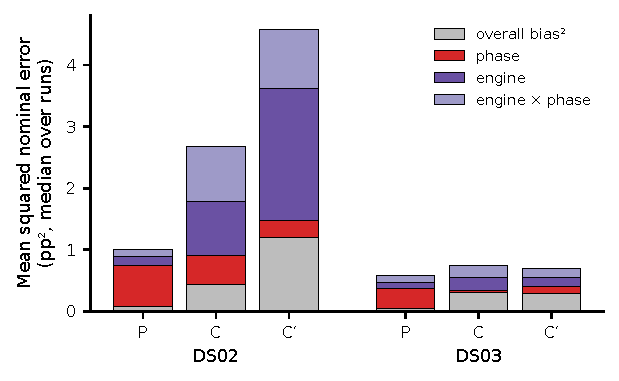
\includegraphics[width=0.65\textwidth]{figures/figS4_error_decomposition.pdf}
\caption{Post-plan descriptive decomposition (Dev-1) of the equal-cell mean squared nominal error at the 1\% target
(median over the seven detector runs).}\label{fig:s4}
\end{figure}

\end{document}
